\documentclass[11pt,a4paper]{article}
\usepackage[margin=1.15in]{geometry}
\usepackage{amsmath,amssymb,amsthm,mathtools}
\usepackage[T1]{fontenc}
\usepackage{microtype}
\usepackage{booktabs}
\usepackage{enumitem}
\usepackage{longtable}
\usepackage{tikz}
\usepackage[hidelinks]{hyperref}

\newtheorem{theorem}{Theorem}[section]
\newtheorem{proposition}[theorem]{Proposition}
\theoremstyle{definition}
\newtheorem{definition}[theorem]{Definition}
\theoremstyle{remark}
\newtheorem{scopenote}{Scope}
\newtheorem{nonclaim}{Non-claim}

\newcommand{\Q}{\mathbb{Q}}
\newcommand{\Z}{\mathbb{Z}}
\newcommand{\R}{\mathbb{R}}
\newcommand{\PP}{\mathbb{P}}

\title{Standard-Model structure from the figure-eight knot complement:\\ what is forced, what is withheld,\\ and what must be supplied}
% ---------------------------------------------------------------------------
% AUTHOR BLOCK -- deliberately a placeholder.
% The repository is public and its privacy rule keeps the owner's name out of
% tracked files, so the author, affiliation and acknowledgements are filled in
% at submission, OUTSIDE the repo. This is not an oversight; removing this
% comment without filling the block would ship an anonymous paper.
\author{[author]\\ \small [affiliation]}
% ---------------------------------------------------------------------------
\date{Draft of 2026-09-09}

\begin{document}
\maketitle

\begin{abstract}
% Provenance (Review 56, R56-10): all verification reported in this paper is internal to the project's own re-runnable pipelines; no external review or endorsement is claimed.
We ask what gauge structure can be extracted from one hyperbolic 3-manifold --- the figure-eight
knot complement $m004$ --- without importing a value. \textbf{We begin with what is generic.} The
$E_6$ recurrence that motivates such programmes is forced by a single ADE classification and is
\emph{not} evidence of specificity; on a census of one-cusped manifolds~\cite{snappy,nz}, roughly one in three admits the
surjection onto the binary tetrahedral group that the construction starts from, and a sibling
sharing the same trace field is not the knot. What survives is narrower and is a theorem of record:
$m004$ is the unique arithmetic knot complement~\cite{reid}, and it is its invariant trace field~\cite{maclachlanreid} $\Q(\sqrt{-3})$
--- a commensurability invariant, distinguished where the group-theoretic scaffolding is not --- that the construction consumes; the
uniqueness itself is load-bearing at no step.

Working from that surviving datum we separate two things a careless account would merge. The object
supplies an \emph{arena} --- a rank-3 abelian sector and a fifteen-dimensional piece of the $27$~\cite{slansky}; that the piece is
\emph{assigned} in Standard-Model-shaped form is an input, listed as such. The \emph{content} is then forced by the anomaly conditions alone, in a computation
containing no token of the object: of $252$ candidate contents, the colour condition alone kills $222$ and the remaining
conditions all but two of the rest. What the object does force is the \emph{termination} of the breaking chain, for
a stated reason, and --- given the colour frame and the Standard-Model shaping that the ledger lists as inputs --- the global form
$[\mathrm{SU}(3)\times\mathrm{SU}(2)\times\mathrm{U}(1)]/\Z_6$ of the Standard-Model factor, an ambiguity the Standard Model
itself does not fix. We then show it
\emph{withholds} values at every bounded-height search we ran: no period of the object survives a $352$-pair comparison with Standard-Model ratios at stated precision (one near-coincidence is dismissed on
three stated grounds), and the hypercharge normalisation is not derivable in principle from the anomaly
equations as algebraic forms.

\textbf{We report the misses.} $\sin^2\theta_W = 3/8$ is the Georgi--Quinn--Weinberg relation~\cite{gqw} reproduced, not
predicted; run to $M_Z$ with gauge-only two-loop running (no Yukawa contribution), Standard-Model content and an assumed desert, it misses as single-step
non-supersymmetric unification is known to miss~\cite{adf,ll}: $\alpha_s = 0.077$ against $0.118$ (a $35\%$ discrepancy),
$\sin^2\theta_W = 0.2293$ against $0.2312$ ($0.9\%$, about fifty experimental standard deviations); the construction's own
closing is supersymmetric, and the supersymmetric crossing has not been run. Three complete copies of the Standard-Model content are \emph{exhibited} on the object's own closings, in mirror pairs,
and they are vector-like: \textbf{the chirality bit is what the object withholds, and we say where, under a stated choice of lift.} Every fixed locus of the
object has even count --- $\chi(\mathrm{Fix}) \in \{0,2\}$, the cusp-fixed and localised counts in $\{0,4\}$ --- and three appears
only through the $\Z/3$ descent, which is vector-like by two conjugations the object or its coefficient field carries. Chirality is not a commensurability invariant: of the object's 87 covers to degree 10, 66 are chiral while the object
is not, and since the invariant trace field is a commensurability invariant those 66 carry a remembered handedness
together with the arithmetic; the spectral wall has held on every sector computed, and the open sectors are the
multi-cusped covers.
No unique four-dimensional field theory follows, and we do not claim uniqueness of the construction.

Finally we list the residue: a freedom ledger with one dimensionful unit that is external by design; two continuous dimensionless anchors, of which one is external \emph{by theorem} --- the object's own modular flow is trivial, so it has no continuous clock to give, and the one route that would import that datum from structure already in hand is exactly tautological; a projective line of Higgs data closed permanently one condition short of a point set, the candidates for that condition having been computed and returned negative; and seven non-continuous rows --- one of which is a relational invariant of a pair, belonging to
neither relatum and requiring no act of selection, while the other six are externally supplied: an
antilinear involution, the seed of a binary label, a choice from a finite menu, the colour frame,
the Standard-Model shaping, and the electromagnetic identification that anchors hypercharge. All verification reported here is internal to the project's own re-runnable pipelines; no external review or endorsement is claimed.
\end{abstract}

\medskip
\noindent\footnotesize
\textbf{Keywords.} arithmetic hyperbolic 3-manifold; figure-eight knot complement; invariant trace
field; binary tetrahedral group; McKay correspondence; exceptional Lie algebra $E_6$; anomaly
cancellation; hypercharge; modular theory; type III factor; chirality; Dehn filling; finite covers.

\smallskip
\noindent\textbf{MSC 2020.} Primary 57K32 (hyperbolic 3-manifolds); Secondary 11F06 (arithmetic
groups), 17B25 (exceptional Lie algebras), 81T50 (anomalies in quantum field theory), 46L36
(classification of factors).

\smallskip
\noindent\textbf{Suggested arXiv classification.} Primary \texttt{math.GT}; cross-list
\texttt{hep-th}, \texttt{math.NT}.
\normalsize

\section{Introduction}

Ask what structure can be extracted from a single mathematical object without importing a physical
measurement, and two failure modes present themselves immediately. The first is to find structure and
overstate what it implies. The second is to find that the structure is generic and quietly not
mention it. This paper is organised to make both difficult.

We therefore invert the usual order. \S\ref{sec:generic} states what is \emph{generic} about the
construction, with the base rates, before any positive claim is made; \S\ref{sec:chain} then lays the derivation out as a chain, link by link, so that a reader can see where its cost actually sits before being asked to accept anything; and \S\ref{sec:unique} states the two facts that survive the genericity. Only then do \S\S\ref{sec:forced}--\ref{sec:observer} say what is forced,
what is provably withheld, and what the residue costs; \S\ref{sec:chirality} does the same for the one bit the Standard Model's spectrum has
and the object's does not. The freedom ledger of
\S\ref{sec:ledger} lists every input the construction requires; a reader who accepts nothing else
should still be able to audit that table, and it is the honest summary of the paper.

The object is the figure-eight knot complement. Its interest here is not that it is a knot
complement, nor that a chain of classifications leads from it to an exceptional Lie algebra --- both
of those turn out to be common. Its interest is that it lies in the one commensurability class an arithmetic knot complement can
occupy; what the chain consumes is that class's invariant trace field $\Q(\sqrt{-3})$, not the manifold's uniqueness, and
the arithmetic, rather than the classification-theoretic scaffolding, is what carries every claim we are prepared to make
(\S\ref{sec:unique} says exactly how much that is).

The result is a boundary rather than a theory. On one side: a gauge algebra with a derived global
form (conditional on two listed inputs), a chain that terminates for a stated reason, and, over chiral matter, a unique
gaugeable abelian direction. On the
other: values that are provably not present, a normalisation that is not derivable in principle, and
a residue that we can price but not eliminate. We end on the second side, in
\S\ref{sec:wall}, because that is where the work actually stops.

\section{What is generic}\label{sec:generic}

We state the base rates first, because a reader's prior on this subject is set by decades of
numerology and because we can measure most of them.

\paragraph{The recurrence is a graph identity.} Programmes of this kind typically observe that $E_6$
recurs across several apparently independent structures --- a McKay correspondence~\cite{mckay}, a Lie classification, a modular-invariant list, a du~Val singularity classification --- and treat the
coincidence as evidence. It is not. Those four are \emph{one} ADE classification presented four ways,
canonically linked; conditioned on the appearance of a single ADE label, the probability that it
``recurs'' across the others is $1$. There is no coincidence to explain.

\paragraph{And the catalogue is short.} $E_6$ is moreover the only exceptional label an imaginary quadratic field can reach, and the
reason is two lines rather than an assertion. A finite subgroup of $\mathrm{SL}(2,K)$ has all of its
traces in $K$. The binary tetrahedral group's traces are $\{0,\pm 1,\pm 2\} \subset \Q$; the binary
octahedral group's include $\pm\sqrt2$ and the binary icosahedral group's include the golden ratio,
so realising either needs $\Q(\sqrt2)$ or $\Q(\sqrt5)$ inside $K$. An imaginary quadratic field
contains no real quadratic subfield but $\Q$. Hence $2O$ and $2I$ --- that is, $E_7$ and $E_8$ ---
are unreachable there, and only $E_6$ remains. So there is not even a birthday problem to argue
about: the space of outcomes has one exceptional element in it.

\paragraph{The entry point is common.} The construction begins with a surjection
$\pi_1(m004) \twoheadrightarrow 2T \cong \mathrm{SL}(2,3)$, of which there are exactly two up to automorphism. That
count is not distinctive, and we give it exactly rather than approximately: over the first $400$ one-cusped
orientable census manifolds in census order, every homomorphism to $\mathrm{SL}(2,3)$ was enumerated over generator images with
no restriction on the presentation and surjections counted up to $\mathrm{Aut}(\mathrm{SL}(2,3)) \cong S_4$:
\textbf{$145$ of $400$ ($36.25\%$) admit such a surjection, and $124$ of $400$ ($31.0\%$) admit exactly two} ---
$m004$'s own count. The class counts that occur are $0$ ($255$ manifolds), $2$ ($124$), $4$ ($14$), $6$ ($4$), $10$
($2$) and $12$ ($1$). \emph{An earlier draft carried two implementations that disagreed by about a percentage
point; the exact count agrees with one of them to the digit and locates the other's defect in a two-generator
restriction, and we record that rather than the tidier version.} The tie list at $m004$'s count begins $m003$,
$m007$, $m022$, $m026$, $m027$, $m029$, $m030$, $m033$, $m034$, $m036$, $m047$ and continues.
Roughly one hyperbolic $3$-manifold in three carries the fact that carries the chain.

\paragraph{The sibling is not the knot, and the coincidence runs deeper than the field.} $m003$
shares the invariant trace field $\Q(\sqrt{-3})$ with $m004$ \emph{and shares its volume exactly}
--- both are $2.0298832128\ldots$ --- without being a knot complement. Both are amphichiral. What
separates them is the cusp shape ($\omega$ for $m003$, in a chosen peripheral basis since it is not a knot complement,
against $2\sqrt3\,i$ for $m004$) --- and, on the record's own re-test, the Chern--Simons invariant, $0$ for $m004$ against
$1/4$ for $m003$ --- neither of which is among the data the
construction's early steps use. So neither the field nor the volume singles out the object. And at the level of grammars rather than manifolds, access to the relevant McKay group is
likewise generic across the metallic family.

\begin{scopenote}[What this does and does not do]
It does \emph{not} break the construction, though the reason is narrower than it first appears. We
do not treat the chain as census-selected: its early steps are constrained to the point where the
population is of size one, so a base rate over manifolds does not falsify them. \textbf{That
constraint is itself conditional on the assumptions of \S\ref{sec:axioms}}, two of which we grade
fragile --- so this defence is available to us only at that stated price. \textbf{What genericity removes is the endpoint's power to confirm the beginning.}
Arriving at $E_6$ is not evidence that the earlier steps were right, if a third of possible entry
points arrive at $E_6$ as well. \emph{The chain can be sound and the Standard Model still fail to
corroborate it.} Every positive claim in this paper is stated under that restriction.
\end{scopenote}

\begin{scopenote}[On our own history]
We did not begin with this discipline. The programme applied base-rate reasoning to numerical
coincidences long before it applied the same test to its flagship structural claim; when the test
was finally run, the structure came back generic. We record that lag because it is the honest
provenance of \S\ref{sec:generic}, and because the rule it produced --- \emph{before treating a
structural recurrence as object-specific, ask whether the faces are canonically linked, how short the
catalogue is, and whether a comparable object shares it} --- is the one we now apply throughout.
\end{scopenote}

\subsection{Assumptions made before the object exists}\label{sec:axioms}

\S\ref{sec:ledger} lists the inputs the construction requires \emph{once the object is in hand}. It
does not list what was assumed to reach the object, and those assumptions are not free. Our own
accounting grades them, and we reproduce that grading rather than paraphrase it:

\begin{itemize}[leftmargin=1.4em,itemsep=2pt]
\item \textbf{A0 --- unpriceable.} The decision to look for structure in a mathematical object at
all. We flag it as permanently philosophical and do not attempt to cost it.
\item \textbf{Four \emph{robust} steps}, which survive every variation we have tried.
\item \textbf{One \emph{geometry-necessary} step}, which cannot be dropped without leaving the
category in which the rest is stated. \emph{(An earlier draft of this list said two robust steps
rather than four, and so enumerated five forks where the accounting it summarises grades seven.
The undercount was found by an external reader; the underlying grading never changed.)}
\item \textbf{Two \emph{fragile} forks}, and we name their discarded siblings because that is what
makes ``fragile'' checkable. The \emph{orientation} fork discards the Gieseking manifold --- which is not a distant
alternative but the non-orientable manifold $m004$ \emph{is} the orientation double cover of, at
exactly half the volume. The \emph{puncture} fork discards a
Sol-geometry mapping torus on which one of the construction's own dynamical faces \emph{survives}.
\end{itemize}

\begin{scopenote}
A reader may reasonably regard the two fragile forks as the place where this construction is most
exposed, and we agree. Nothing in this paper argues that the forks were forced; what is argued is
that \emph{given} the object they select, the consequences in
\S\S\ref{sec:forced}--\ref{sec:observer} follow.
\end{scopenote}

\section{The chain, link by link}\label{sec:chain}

Everything above is organised by \emph{kind} of claim. This section does the other thing a reader
needs and states the derivation as a \textbf{chain}, in order, with each link carrying its own type.
We do this because the interesting fact about the chain is not its length but \emph{where its cost
sits}, and that is invisible until the links are laid out.

There are \textbf{fifty-four links}. Their types are: thirty-four theorems, six identities, eight
no-go results, one census, one corollary --- and \textbf{four axioms}. So fifty of fifty-four
links are forced, in the precise sense that they are not declared choices.

\paragraph{Where the four axioms are, which is the point.} They are not distributed through the
derivation. They sit at the two ends:

\begin{itemize}
\item \textbf{Three before the object exists} --- that being is inexhaustible description; that the
word is realised on a geometric carrier; and \emph{orientation}, which our own accounting marks the
most expensive of the three.
\item \textbf{One after the algebra is in hand} --- the observer's closings.
\item \textbf{Between the manifold and the observer's axiom: none} (Figure~\ref{fig:chain}). Across the twelve consecutive
links $6$--$17$ --- the manifold's realisation, its own arithmetic and spectral structure, and two no-go results --- there is
\textbf{not one declared choice.} Two honesty notes on the shape. The exceptional algebra is not a numbered link in that
stretch: it is handed over by the McKay correspondence, a theorem that requires no choice, and its explicit construction is
certified at link $26$. And the measurement links $24$--$42$ carry numbers after the observer's axiom $18$ because they were
banked later, not because they depend on it: they are exact algebra on the object's own charges. We state the shape as the
table carries it and do not claim a dependency order the table does not.
\end{itemize}

\begin{scopenote}
We state the consequence in the form we can defend, and no stronger. This is \emph{not} a claim that
the construction is parameter-free; it is the claim that \textbf{its parameters are enumerated,
typed, and located} --- three at the entrance, one at the exit, none in the middle. A reader who
rejects any of the four is entitled to reject what follows from it, and can see exactly what that is.
The post-object continuous inputs are separately tabled in \S\ref{sec:ledger}; of those, one is
external by theorem, one is closed permanently subject to a single named datum, and the rest are
finite labels.
\end{scopenote}

\begin{scopenote}[Two accountings, and they are the same cost]
\S\ref{sec:axioms} prices the entrance as seven forks of which two are fragile; this section prices
it as four axioms of which three precede the object. These are not rival counts. \textbf{The forks
are how the axioms are priced}: the description axiom is priced by two forks that both return
robust, the carrier axiom by the redundancy analysis that fails in four independent ways, the
orientation axiom by the fork that returns fragile, and the observer's closings by four further
forks of their own. A reader who wants the cost in one number should take the axioms; a reader who
wants to know how hard each was pushed should take the forks.
\end{scopenote}

\begin{figure}[h]
\centering
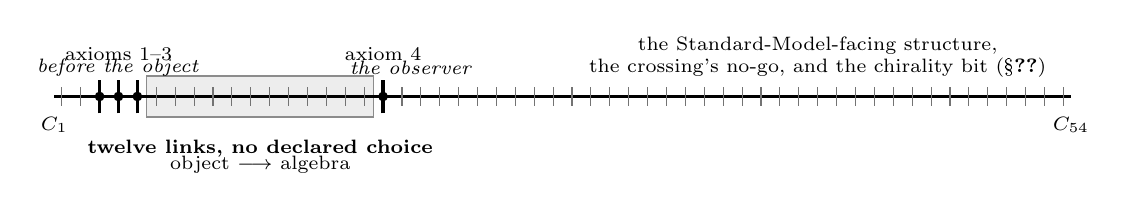
\begin{tikzpicture}[x=2.4mm,y=1mm]
  % the axiom-free stretch, shaded
  \fill[black!7] (5.5,-2.6) rectangle (17.5,2.6);
  \draw[black!45] (5.5,-2.6) rectangle (17.5,2.6);
  % the chain
  \draw[thick] (0.6,0) -- (54.4,0);
  \foreach \i in {1,...,54} \draw[black!55] (\i,-1.15) -- (\i,1.15);
  % the four axioms
  \foreach \i in {3,4,5,18} {
    \draw[very thick] (\i,-2.15) -- (\i,2.15);
    \fill (\i,0) circle (0.62mm);
  }
  \node[font=\scriptsize] at (4,5.4) {axioms 1--3};
  \node[font=\scriptsize] at (4,3.6) {\emph{before the object}};
  \node[font=\scriptsize] at (18,5.4) {axiom 4};
  \node[font=\scriptsize] at (19.5,3.6) {\emph{the observer}};
  \node[font=\scriptsize] at (11.5,-6.6) {\textbf{twelve links, no declared choice}};
  \node[font=\scriptsize] at (11.5,-8.6) {object $\longrightarrow$ algebra};
  \node[font=\scriptsize] at (0.6,-3.6) {$C_1$};
  \node[font=\scriptsize] at (54.4,-3.6) {$C_{54}$};
  \node[font=\scriptsize,align=center] at (41,5.0) {the Standard-Model-facing structure,\\ the crossing's no-go, and the chirality bit (\S\ref{sec:chirality})};
\end{tikzpicture}
\caption{\small The chain's fifty-four links, with each of the four axioms marked. The point is
the \emph{shape}: the cost is not spread through the derivation but sits at the two ends, and the
shaded stretch, links $6$--$17$ --- the manifold's own structure --- contains no declared choice at all; the algebra is
handed over by McKay, and the measurement links follow the observer's axiom in numbering, not in dependence.
Fifty links are forced. The crossing's no-go sits where it fell, and the chain now runs past it to the
chirality bit.}
\label{fig:chain}
\end{figure}


\paragraph{The links themselves.} Two readers of an earlier draft made the same objection, and it
was correct: the chain is what this paper claims to have, and stating only its \emph{shape} while
withholding its contents asks for trust exactly where the paper offers audit. So the links are
below. The tally beneath the table is recomputed from the table, not copied from the paragraph
above it, and the table itself is generated from the ledger rather than typed --- which is how two
mis-parses were caught while preparing it, each of which had produced a link count disagreeing with
the prose it was meant to support.

% ---- GENERATED by scripts/checks/paper_chain_table.py --tex ; do not hand-edit ----
\begingroup\footnotesize
\setlength{\LTleft}{0pt}\setlength{\LTright}{0pt}
\begin{longtable}{@{}r l p{8.2cm}@{}}
\textbf{\#} & \textbf{Type} & \textbf{Link} \\ \midrule \endhead
1 & Theorem & every aperiodic sequence has factor complexity $\ge$ n+1, and Sturmian words attain it (Morse-Hedlund) \\
2 & Theorem & the self-similar Sturmian slopes are the quadratic class (theorem); among them the minimal-description criterion selects the golden slope (the criterion of link 3, split at link 53) \\
3 & \textbf{AXIOM} & being is inexhaustible description; PRICED by the periodic and shadow-rule forks \\
4 & \textbf{AXIOM} & the word is realised on the once-punctured torus; PRICED (the combinatorial carrier reaches only Q(sqrt5)) \\
5 & \textbf{AXIOM} & orientation: the monodromy is the golden matrix squared; PRICED, the discarded sibling is the Gieseking manifold \\
6 & Theorem & the mapping torus of $[[2,1],[1,1]]$ is the figure-eight knot complement, invariant trace field Q(sqrt-3) (Thurston, Riley) \\
7 & Theorem & the intrinsic arithmetic forces exactly three quadratic faces, Q(sqrt-3), Q(sqrt5), Q(sqrt-15), one Klein four-group \\
8 & Census & no closed filling in the |p|,q $\le$ 8 grid carries any of the three faces: the faces belong to the open object \\
9 & Theorem & the manifold group is congruence (level 4 in the SL-kernel convention; geometric index 12 at level 8) \\
10 & Theorem & character rigidity: the continuous spectrum is one channel, $\varphi(s)$ = $\Lambda_K(s-1)/\Lambda_K(s)$ exactly \\
11 & Identity & the two-column law: ten of twelve structural floors carry a forced golden appearance, the emission channel none \\
12 & Theorem & the trace map is theta-equivariant and the odd golden powers sit in the theta-odd sector (dominant $\varphi^3$) \\
13 & Identity & the theta-odd block at the monodromy is unitary with eigenphases $\pm$72 deg; the overlap matrix is golden-exact \\
14 & Identity & the symmetrised Kashaev series has pure-3 denominators through fifth order \\
15 & Theorem & the mod-5 generating function is multiplicative exactly on a quadratic-residue condition \\
16 & No-go & every refusal to close falls into three classes: no point, no width, no name \\
17 & No-go & zero of the 24 Standard-Model parameters is reduced by the spectral route; two live claims dissolved \\
18 & \textbf{AXIOM} & the observer's closings (chirality, values, time, the spatial manifold) are choices; four forks priced \\
19 & Identity & the theta-off-block norm at the geometric representation equals the geometric pair's separation \\
20 & Identity & the observer's discrete closing set has $\mathbb{F}_2$-rank exactly 3 (conjugation, reversal, the golden Galois branch) \\
21 & Theorem & the unmoved axis is a discrete 3-element torsor with no continuous modulus \\
22 & Corollary & the closing set is a torsor, hence has no canonical point (corollary) \\
23 & No-go & no object-native operation moves the frame: the realised subgroup of Out(V\_4) is trivial \\
24 & Theorem & the first measurement: at each of the three noncompact walls the centraliser is so(10) + u(1) \\
25 & Theorem & the second measurement lands on su(3) + su(2) + $\mathfrak{u}(1)^3$, the A\_2 + A\_1 Levi subalgebra (dimension 14, rank 6: two abelian factors beyond the Standard Model) \\
26 & Theorem & the constructed algebra is the magic-square algebra M(O, C): a Lie isomorphism on all 3003 unordered basis pairs, zero mismatches \\
27 & Theorem & the inter-breaking laws on the matter pencil (vacuum to Higgs; the 16/vacuum exclusion) \\
28 & Theorem & measured walls = theta-odd exponents (4, 8), unmeasured = (7, 11); the resolvent field is Q(sqrt77), disc K = $3^4\cdot 7\cdot 11$ \\
29 & Theorem & the signature dichotomy: the two noncompact charges are real-spectrum, the two compact ones imaginary \\
30 & Theorem & the sign law of the torsion quotients: all six anti-palindromic with sign fixed by parity \\
31 & Theorem & the diagonal cocycle: all four label cubics have a root in K, one root permutation for both orbits \\
32 & No-go & no real C-stabilising symmetry swaps split and compact: the carrier of c must be complex \\
33 & Theorem & the annihilation: vacuum class times charge class is trivial (vacuum + charge = the split algebra) \\
34 & Theorem & one Kummer class spans the structure and value layers; the observer's place is a degree-one prime of K \\
35 & Theorem & the generation shape: flavour triplets replicate fixed colour x su(2) types (sealed cell) \\
36 & Theorem & one Z\_2-graded law: matter gluing = gauge commutation = mixed texture type; fifteen flavour atoms \\
37 & Theorem & the real form selected by the wall is e\_6(2) \\
38 & Theorem & the four charges commute rationally on the 27; the invariant ratio is I = -1 \\
39 & Theorem & the canonical Hermitian form on the 27 has signature $(15,12)$ \\
40 & Theorem & the six normalisation-free colourless couplings are one number \\
41 & Theorem & the coupling normalisation is 1 in the charge-equivariant gauge; v\_1 v\_2 v\_3 = $3^{3/2}$ times its square; structure primes inert, value primes split \\
42 & Identity & $\mathrm{Tr}(T_3^2) = 3$, $\mathrm{Tr}(Y^2) = 5$, $\mathrm{Tr}(T_3 Y) = 0$ on the 27: the 3/8 trace ratio, as structure \\
43 & No-go & the sealed one-input crossing to measured values misses as single-step non-supersymmetric unification is known to ($\alpha_s$ by 35\%, $\sin^2\theta_W$ by 0.9\%); the desert is dead as a mechanism \\
44 & No-go & the fork: the joint centraliser of spacetime, colour and hypercharge is zero -- any two, never three \\
45 & No-go & every anomaly channel vanishes identically over the derived 16 with $\nu^c$: anomaly matching constrains nothing further \\
46 & Theorem & closing is constitutive: ten exceptional fillings, the fibre slope the unique torus bundle with monodromy LR, and no closed filling keeps Q(sqrt-3) \\
47 & Theorem & the parity of the cusp \\
48 & Theorem & every fixed locus counts two or nothing \\
49 & Theorem & the charge-locus parity lock, and the lift fork \\
50 & Theorem & the one-cusped index, and the cyclic tower is vector-like \\
51 & Theorem & the tower law and the Standard-Model closings \\
52 & No-go & the $\theta$-odd frame is closed on every sl$_2$ germ \\
53 & Theorem & the genesis dictionary, the criterion census, and the substrate fork \\
54 & Theorem & the mirror is swap $\times$ arrow, and covers do not inherit amphichirality \\
\end{longtable}\endgroup

\noindent\footnotesize Recomputed from the table above rather than asserted:
34 theorem, 8 no-go, 6 identity, 4 axiom, 1 census, 1 corollary, totalling 54 links, of which \textbf{50} are not axioms. The four axioms are
links 3, 4, 5, 18 --- three before the object exists and one after the
algebra is in hand --- and \textbf{no link between 6 and 17 is an
axiom}, which is the twelve-link stretch this section is about.\normalsize
% ---- end generated chain table ----

\paragraph{The entrance: from ``not nothing'' to a word.} The first two links are borrowed
mathematics, not ours. Morse--Hedlund~\cite{morsehedlund} fixes what an aperiodic sequence must cost in
factor complexity; extremality in the Hurwitz sense~\cite{hurwitz} then selects, by a single criterion, the golden case.
What this buys is modest and we say so: a distinguished \emph{word}, not yet a space. The step from
the word to a space is the second axiom, and the step from a space to an \emph{oriented} space is
the third.

\paragraph{The bridge from the word to the manifold is an identity, and it is exact.} Let $M$ be the
substitution matrix of the golden rule $a \mapsto ab$, $b \mapsto a$. Then
\[
M^2 \;=\; \begin{pmatrix}2&1\\1&1\end{pmatrix} \;=\; LR,
\]
where $L = \bigl(\begin{smallmatrix}1&1\\0&1\end{smallmatrix}\bigr)$ and
$R = \bigl(\begin{smallmatrix}1&0\\1&1\end{smallmatrix}\bigr)$ are the two shears in the record's naming ($LR$ and $RL$ are
conjugate in $\mathrm{GL}_2(\Z)$, which is exactly why the commensurability class forgets the order and the bit below is
carried by the swap's placement inside the generating step), and $LR$ is precisely the monodromy of the once-punctured torus bundle whose mapping torus is our
manifold. \textbf{The golden substitution matrix, squared, is the object's monodromy.} The squaring
is not cosmetic: it \emph{is} the orientation axiom. The un-squared matrix gives a non-orientable
manifold of exactly half the volume --- and that manifold is not a distant alternative but the one
our object double-covers. This is why we grade the orientation axiom the most expensive: its
discarded sibling is the nearest possible neighbour.

\paragraph{The exit from the arithmetic, and a limit we must state.} The combinatorial layer
delivers the golden field and \emph{only} the golden field. Four independent routes were
pre-registered to test whether the quadratic field carrying the exceptional algebra could be reached
from the combinatorial data alone, and \textbf{all four fail}: the relevant polynomial stays
irreducible over the golden field (against a control that does split correctly), the gap labels stay
in the golden ring, cone preservation pins the endomorphism ring, and no three-torsion appears.

\begin{scopenote}
The consequence is a boundary, and it is one of the sharper things this programme knows about
itself: \textbf{the second field is bought at geometrization and nowhere earlier.} The combinatorial
and substitution-theoretic layer cannot reach it. So the golden end and the exceptional end of this
construction are not two faces of one arithmetic --- they are separated by exactly the step that
turns a word into a hyperbolic manifold.
\end{scopenote}

\paragraph{The middle: twelve links and no choices.} What follows the manifold is where the
derivation earns its keep, and it is the stretch with no axioms in it: the mapping torus is realised as the hyperbolic manifold~\cite{thurston}; its intrinsic arithmetic forces its three quadratic faces; the interface structure is
settled by an exhaustive census rather than a selection; congruence is established with its
conventions named; character rigidity fixes the spectrum; the trace map's $\theta$-equivariance and the golden-exact mixing
block follow; and the stretch closes on two no-go results about what the object refuses. \S\ref{sec:middle} states each.

\paragraph{How the exceptional algebra arrives.} It is worth being exact about this, because a
weaker version of the argument was withdrawn and the weaker version is the one a reader is likely to
guess. The algebra is \textbf{not} obtained by factoring a congruence level into coprime parts --- we
tried that reading, it is false (the level in question is irreducible), and it was retracted. What is
true is geometric: the binary tetrahedral group sits at the object's \emph{hyperbolic} end and hands
over the exceptional algebra by the McKay correspondence, exactly as the binary icosahedral group
sits at the \emph{spherical}, golden end and hands over the larger one. The algebra follows from the McKay correspondence applied at the hyperbolic end, and which one arrives is fixed by
which curvature end one stands at; by \S\ref{sec:generic}'s base rate the entry point is not object-specific, so
this step is not evidence for the object.

\paragraph{The exit: the observer, then the wall.} The fourth axiom enters only here, after the
algebra is in hand, and \S\ref{sec:observer} prices it. What follows it is the Standard-Model-facing
structure --- the measurement layer, the magic-square isomorphism, the selection of the real form,
the generation shape, the trace identities~\cite{fricke} --- and the chain ends where this paper ends, on a no-go:
the crossing to measured values, sealed and negative --- the known failure of desert unification, reproduced on the
object's boundary value.

\paragraph{The shape of the journey, stated plainly.} A reader who wants the whole route in one sentence should have it in
the form we can defend. From the word to the manifold the derivation is exact and is the object's (the entrance, the
squaring, the geometrization). From the manifold through its own structure it is forced and is the class's, not the manifold's: the twelve links are
theorems about the commensurability class of $\Q(\sqrt{-3})$ and about the golden substitution; the algebra is then handed
over by McKay, and the entry to it is one a third of census manifolds share. From the algebra to the Standard-Model \emph{arena} the object supplies
part of the arena and the observer the rest (\S\ref{sec:ledger}). From the arena to the \emph{content} the object
supplies nothing: the anomaly conditions do that work alone (\S\ref{sec:forced}). And from the content to a chiral
spectrum the object supplies the count two and withholds the bit (\S\ref{sec:chirality}). Two of the five legs are
the object's own; the paper's result is the location of the other three.

\begin{scopenote}[Recorded in advance]
The chain terminates in a \emph{negative} link and we have not hidden it in the middle. A reader
should take the shape seriously: a derivation that reaches Standard-Model \emph{structure} through
fifty forced links and then fails, provably and by its own sealed criterion, to reach
Standard-Model \emph{values}, is reporting something about where the boundary between the two lies.
That boundary is what the freedom ledger of \S\ref{sec:ledger} prices.
\end{scopenote}

\section{What is unique}\label{sec:unique}

Two facts survive \S\ref{sec:generic}. Everything this paper claims is built on them and on nothing
else.

\paragraph{Arithmeticity --- and it is a statement about the class, not the manifold.} Among knot
complements, $m004$ is the \emph{unique} arithmetic one. That is a theorem of the literature and it
is true, but \textbf{we must be careful about what our construction actually consumes}, and it is not
that uniqueness.

What the chain buys is the \emph{invariant trace field} $\Q(\sqrt{-3})$ --- and the invariant trace field is a
\emph{commensurability-class} invariant, not a manifold invariant. The sibling $m003$ carries the
same field and the same volume (\S\ref{sec:generic}); it is not separated from $m004$ by anything the
chain purchases. Knot-ness enters exactly once, and as a \emph{discriminator} rather than a
foundation: $H_1(m003) = \Z/5 \oplus \Z$ against $H_1(m004) = \Z$.

\begin{scopenote}
So the honest form of this paper's positive content is: \textbf{a theorem about the commensurability
class of $\Q(\sqrt{-3})$, joined to a theorem about $E_6$ by a generic fact.} It is strong as a
statement about the class and weak as a statement about $m004$ in particular, and we state it the
first way. Uniqueness of the arithmetic knot complement is load-bearing at no step of the
construction; we cite it because it is true and relevant, not because anything rests on it.
\end{scopenote}

\paragraph{A uniqueness at the level of grammars.} The second is ours, and it is a proof over an
infinite family rather than a census --- conditional on one stipulated definition, stated below.

\begin{proposition}\label{thm:golden}
Call $G$ \emph{binary polyhedral} if $G \in \{2T, 2O, 2I\}$ (orders $24$, $48$, $120$), and define the \emph{level} of the
metallic grammar $R^mL^m$ ($m \ge 1$) to be $\Lambda(m) := m^2 + 4$, the discriminant of its characteristic polynomial divided
by $m^2$. Then exactly one metallic grammar has level equal to a modulus $N$ for which $\mathrm{SL}(2,\Z/N)$ is binary
polyhedral: the golden grammar $m = 1$, with $N = 5$ and $\mathrm{SL}(2,\Z/5) \cong 2I$.
\end{proposition}

\noindent The statement is conditional on that normalisation of ``level'', which is stipulated here rather than derived from
an intrinsic congruence level, and we say so before the proof rather than after it. Note also which end selects: $m = 1$ is
singled out by the modulus $5$ and the binary icosahedral group --- the golden, spherical end of the object, $E_8$'s --- and
not by the $2T$ that hands over $E_6$ at the hyperbolic end.

\begin{proof}
Two independent facts meet once. First, $\mathrm{SL}(2,\Z/N)$ \emph{is} a binary polyhedral group for exactly $N \in \{3,5\}$:
$\mathrm{SL}(2,\Z/3) \cong 2T$ and $\mathrm{SL}(2,\Z/5) \cong 2I$, giving $E_6$ and $E_8$.
\textbf{The case $N=4$ is an order coincidence and not an isomorphism, and we flag it rather than
count it}: $|\mathrm{SL}(2,\Z/4)| = 48 = |2O|$, but the reduction
$\mathrm{SL}(2,\Z/4) \to \mathrm{SL}(2,\Z/2) \cong S_3$ has kernel $\cong (\Z/2)^3$, in which every
element is an involution, so $\mathrm{SL}(2,\Z/4)$ has \emph{seven} elements of order two. Every
binary polyhedral group embeds in the unit quaternions, where $-1$ is the unique involution. Hence
$\mathrm{SL}(2,\Z/4) \not\cong 2O$, and it is not binary polyhedral at all. \emph{This is precisely
the short-catalogue coincidence this paper's own method section refuses to treat as evidence, and we
were caught treating it as evidence here.} Completeness here is a proof and
not a bounded search: from
\[
  |\mathrm{SL}(2,\Z/N)| \;=\; N^3\!\!\prod_{p \mid N}\!\left(1 - \tfrac{1}{p^2}\right)
  \;\ge\; N^3 \prod_{p}\left(1 - \tfrac{1}{p^2}\right) \;=\; \frac{N^3}{\zeta(2)} \;=\; \frac{6}{\pi^2}N^3 ,
\]
and $\tfrac{6}{\pi^2}N^3 > 120$ for every $N \ge 6$ (at $N=6$ already $131.3 > 120$), no modulus
beyond $5$ can even reach the required order. The two small moduli are disposed of directly:
$|\mathrm{SL}(2,\Z/1)| = 1$ and $|\mathrm{SL}(2,\Z/2)| = 6$. So the admissible list is
$N \in \{3,5\}$, complete, with no case left unexamined. Second, write $\Lambda(m) := m^2+4$. This is the \emph{level} of the metallic grammar
$R^mL^m$, not its field conductor: $\mathrm{tr}(R^mL^m) = m^2+2$, so the discriminant of its
characteristic polynomial is $m^2(m^2+4)$ and $\Lambda(m) = D/m^2$. \textbf{The distinction is not
cosmetic.} Under the field-conductor reading the statement would be false --- $m = 4, 11, 29$ all
give $\Q(\sqrt5)$ and hence reach $|2I| = 120$ --- and it is the level, not the conductor, that the
argument requires. Setting $\Lambda(m)$ equal to each admissible modulus with $m \ge 1$: $m^2+4 = 3$ has no solution and $m^2+4 = 5$
gives $m = 1$. \qedhere
\end{proof}

\noindent Only two moduli qualify, not three, so there is no three-way coincidence here to note or to
decline --- and the $N=4$ near-miss is a caution rather than a pattern. What the theorem supplies is narrow and real: a uniqueness
that survives \S\ref{sec:generic}, obtained over an infinite family, at the opposite end of the
construction from the census whose base rate defeated the earlier claim.

\paragraph{An outside meeting point.} Independently of this programme, a mixed Tate motive has been constructed~\cite{lee} for finite-volume hyperbolic $3$-manifolds whose Beilinson regulator is the complex
volume, defined over the invariant trace field --- which for $m004$ is exactly $\Q(\sqrt{-3})$ --- with
the figure-eight complement as a verified case. We record it as corroboration that the arithmetic
datum, rather than the ADE scaffolding, is the load-bearing one.

\section*{Non-claims}
This paper does \emph{not} claim:
\begin{nonclaim} to derive the Standard Model. \end{nonclaim}
\begin{nonclaim} to predict any measured value. \end{nonclaim}
\begin{nonclaim} that the object is the universe, or a model of it. \end{nonclaim}
\begin{nonclaim} that three \emph{chiral} generations are derived. Three structural copies of the Standard-Model content
are exhibited on the object's own closings, in mirror pairs; they are vector-like, and \S\ref{sec:chirality} proves at every computed
sector where the chirality bit is withheld. \end{nonclaim}
\begin{nonclaim} that the sign pattern of the object's symmetries (the mirror is the swap times the arrow,
\S\ref{sec:chirality}) is the Standard Model's $C$, $P$, $T$ pattern. It is a resonance we record and do not claim. \end{nonclaim}
\begin{nonclaim} that $\sin^2\theta_W = 3/8$ is a prediction. It is the Georgi--Quinn--Weinberg relation~\cite{gqw}, reproduced; run down across an assumed desert it misses as
non-supersymmetric single-step unification is known to~\cite{adf,ll}: $\alpha_s$ by $35\%$, $\sin^2\theta_W$ by $0.9\%$. The
running is imported Standard-Model dynamics, not anything the object supplies. \end{nonclaim}
\begin{nonclaim} that any dynamics, rate, or action is supplied. \end{nonclaim}
\begin{nonclaim} that the observer's bit is consciousness, or that it is not. \end{nonclaim}
\begin{nonclaim} that every one of the chain's fifty forced links is stated in this paper in checkable form: \S\ref{sec:chain}
states the entrance, the twelve middle links and the walls in full; the measurement and value links are stated there in one
line each and in the records the appendix names. \end{nonclaim}
\begin{nonclaim} that the global-form selection is independent of the colour frame and the Standard-Model shaping; it is
conditional on both, and \S\ref{sec:ledger} lists them as inputs. \end{nonclaim}

\section{The middle of the journey: from the manifold to the algebra, and from the algebra to the arena}\label{sec:middle}

The chain of \S\ref{sec:chain} named its links; this section states the ones a reader cannot follow from a name. It is
the part of the route that is the object's own --- the twelve links with no declared choice, then the algebra, then the
calculus by which the object's charges are measured down to the Standard-Model arena --- and it is written so that a reader
who accepts \S\ref{sec:generic}'s restriction can still see what, concretely, the manifold forces. Every statement below is
established in a re-runnable record, and the appendix names one for each load-bearing claim; none is new here. Throughout this
section C$n$ means link $n$ of the table in \S\ref{sec:chain}, and \emph{the record} means the project's re-runnable record to
which the appendix maps each claim.

\paragraph{What the manifold forces about itself.} The manifold's intrinsic arithmetic forces exactly three quadratic
faces --- $\Q(\sqrt{-3})$, the invariant trace field; $\Q(\sqrt5)$, the field of the golden dilatation; and their compositum's
third quadratic subfield $\Q(\sqrt{-15})$ --- one Klein four-group, and no fourth (C7). A census over the $78$ hyperbolic
fillings of the $|p|,q \le 8$ grid finds \emph{no} closed filling whose invariant trace field contains any of the three
(C8): the faces are a property of the \emph{open} object, and closing it loses them. The manifold group is congruence
(level $4$ in the $\mathrm{SL}$-kernel convention, geometric index $12$ at level $8$; C9) --- a statement that defies Serre's
non-congruence base rate, computed twice on our own benches and not yet checked against the literature. Its continuous spectrum
is a single channel: the pullback Eisenstein series, with scattering determinant $\varphi(s) = \Lambda_K(s-1)/\Lambda_K(s)$ for
$K = \Q(\sqrt{-3})$ exactly and no conductor character anywhere in the continuous part (C10; for the weight-zero scalar
Laplacian, with three classical inputs cited rather than re-proved). And the trace map of the
genesis is $\theta$-equivariant, with the odd golden powers in the $\theta$-odd sector (C12), where the $\theta$-odd block of
the twisted transfer operator at $g = RL$ is exactly unitary with eigenphases $\pm 72^\circ$ (the untwisted operator gives
$\pm 108^\circ$) and the overlap between the forced weight basis and
its eigenbasis is the golden-exact, twist-invariant unistochastic matrix
$\bigl[\begin{smallmatrix}\varphi/\sqrt5 & 1/(\varphi\sqrt5)\\ 1/(\varphi\sqrt5) & \varphi/\sqrt5\end{smallmatrix}\bigr]$
(C13). The other six of the twelve are one-line entries in the table --- the two-column law (C11), the pure-$3$ symmetrised
series (C14), the mod-$5$ multiplication law (C15) --- and the stretch closes on its two no-go links: every refusal to close
falls into three classes (C16), and zero Standard-Model parameters are reduced by the spectral route (C17). These are the
twelve links' content: theorems about the commensurability class of $\Q(\sqrt{-3})$ and about the golden substitution, none
of them a choice.

\paragraph{How the algebra arrives, exactly.} The binary tetrahedral group $2T \cong \mathrm{SL}(2,3)$ is a quotient of the
manifold group (\S\ref{sec:generic} gives the base rate of that fact); by the McKay correspondence its representation graph
is the affine $E_6$ diagram, and the exceptional algebra is read off. The construction then builds the algebra explicitly
from the four-element charge torus $\mathfrak{z}(2T) = \mathfrak{u}(1)^4$, the centraliser in $\mathfrak{e}_6$ of the
holonomy's binary tetrahedral image, and the build is certified against the classical one: it \emph{is}
Barton--Sudbery's magic-square algebra $M(\mathbb{O},\mathbb{C})$~\cite{bartonsudbery}, verified as a Lie isomorphism on all
$3003$ unordered basis pairs with zero mismatches (C26); the minimal module is the $27$, the exceptional Jordan algebra, with its cubic invariant.
The structural theorem of that layer is the one this paper's title turns on: \textbf{the object forces form, not values} --- the
Galois group of the object's own arithmetic (on the value layer, the $S_3$ of the cubic field $K$ below) acts on every quantity
the algebra produces, so the object fixes orbits and never points (the ``Galois firewall'' of the record, and the reason
\S\ref{sec:withheld} exists as a separate instrument).

\paragraph{The measurement calculus: how the arena is derived rather than stipulated.} The four charges of the torus are not
a basis choice; they carry canonical geometry. Their Killing Gram matrix is diagonal with signature $(2,2)$: one pair is
noncompact and one compact, and the determinant is a perfect square. The fifteen coordinate subtori of the four charges have
centralisers of only two dimensions --- $30$ for the three subtori inside the noncompact pair, $12$ for the twelve that touch
the compact pair --- and the $30$ is the $\mathfrak{so}(8) \oplus \mathfrak{u}(1)^2$ triality core; three further,
non-coordinate charge lines, $S_3$-conjugate, have $46$-dimensional centralisers. The two censuses are over different sets and
we keep them apart. The only sign flips that survive form a Klein four-group. Each pair degenerates along a cubic pencil; the two cubics have Galois group $S_3$ and the \emph{same}
resolvent field $\Q(\sqrt{77})$, and they generate a single cubic field $K$ of discriminant $3^4 \cdot 7 \cdot 11$ (C28).
\emph{Measuring} at a wall means passing to the centraliser of the charge there. At each of the three non-coordinate lines the
centraliser is $\mathfrak{so}(10) \oplus \mathfrak{u}(1)$ --- three $S_3$-conjugate charge lines tiling the algebra (C24,
the first measurement); inside the compact pair it is the $\mathfrak{so}(8) \oplus \mathfrak{u}(1)^2$ core; and the most
generic non-trivial second measurement lands on $\mathfrak{su}(3) \oplus \mathfrak{su}(2) \oplus \mathfrak{u}(1)^3$
exactly, the $A_2{+}A_1$ Levi, skipping $\mathrm{SU}(5)$ over $\R$ --- over the algebraic closure the
$\mathrm{SU}(5) \times \mathrm{U}(1)$ stratum is attained at four non-real points, so the skip is a reality phenomenon,
and the wall point's reality is supplied by the closing \S\ref{sec:ledger} lists (C25, the second measurement). That algebra is rank six, not four: two
abelian factors beyond the Standard Model's remain, and \S\ref{sec:withheld} says what becomes of each. The matched and
mismatched measurements generate the classical chain $12 \subset 18 \subset 30 \subset 46 \subset 78$. This is $E_6$'s own
structure, computed in the charge frame the holonomy supplies --- the four-element torus is the object's, the centraliser lattice
is the algebra's, and \S\ref{sec:recognition} records that the landing algebra itself is classical --- and it is exactly what
\S\ref{sec:forced} then subtracts from: which of the three $A_2$'s is colour, and the Standard-Model shaping of the multiplet,
are not selected by any of it.

\paragraph{The matter law, and what it is not.} Under the $\mathfrak{so}(10)$ the first measurement produces, $27 = 16 + 10
+ 1$: one complete Standard-Model generation with a right-handed neutrino, two Higgs doublets with the exotic colour-triplet
pair, and a singlet. The couplings obey one $\Z_2$-graded law --- $[E_i, E_j] = 0$ exactly when $s_i s_j = c_{ij}$ ---
verified on four faces (gauge commutation, matter gluing $32/32$, the mixed Yukawa type $48/48$ under seal, the atomic census
$8/8$ under seal), with $\prod c = -1$ the obstruction; the $27$ tiles into fifteen pieces uncuttable by all three
labellings at once, and the colourless coupling grid is $K_{3,3}$ (C36). What this is \emph{not}: a generation count.
An earlier reading named a triplet index of this structure ``flavour''; what was tested and refuted is that name --- the index is
trinification structure, not generation structure --- and the paper does not use it. The cubic field's three branches remain the
record's index for the coupling hierarchy below, and ``the three-element index'' there means that and nothing more.

\paragraph{The value layer the object does have.} \S\ref{sec:withheld} proves that none of the object's numbers is a
Standard-Model value. It would be misleading to leave the impression that the value layer is empty, so we state what it
holds, all of it structure. Of $128$ involution classes exactly two make the matter wall real, and both are the quaternionic
form $\mathfrak{e}_{6(2)}$ --- a pre-registered computation whose disclosed prior had been $\mathfrak{e}_{6(-14)}$, and which
overruled it (C37). The
canonical Hermitian form on the $27$ has signature $(15,12)$, the $\mathfrak{su}(6) \oplus \mathfrak{su}(2)$ split (C39).
The four charges commute rationally on the $27$ and the invariant ratio of row and column products is $I = -1$ exactly, as an
identity of exact integers with no height bound (C38). The nine coloured-line couplings factor as $\Lambda = v \otimes v$ over
a three-element index, and in the $\tau$-twisted gauge the three values are the Galois conjugates of one element of $K$,
$v_g^2 = V(\rho_g)$, with $v_1 v_2 v_3 = 3^{3/2}\mu^2$ for $\mu = 2304/953$; in the charge-equivariant gauge the
normalisation is $\mu = 1$ exactly and the three values collapse to a triple root, the whole hierarchy being carried by the
Hermitian twist (C40, C41). We attach no flavour reading to the index and quote no ratio. In the normalisation
$Q = T_3 + Y$ (so that $Y$ is half the conventional hypercharge), $\mathrm{Tr}(T_3^2) = 3$, $\mathrm{Tr}(Y^2) = 5$ and
$\mathrm{Tr}(T_3 Y) = 0$ on the $27$, so $\sin^2\theta_W = 3/8$ (C42); the ratio is the same on the $5$, $\bar 5$, $10$ and
$16$, so it is a property of the $\mathrm{SU}(5)$-compatible embedding and not of the $27$, it discriminates nothing about the
object, and the anchoring of $Y$ by $Q = T_3 + Y$ is an identification the ledger lists as an input --- which is why
\S\ref{sec:recognition} calls the Georgi--Quinn--Weinberg relation reproduced and not assumed. All of this is physics-shaped and none of it is
physics-valued: it is the form the Galois firewall permits.

\paragraph{The three crossings.} The construction was carried to the measured world under seal three times, and all three
outcomes are on the record. The first (\S\ref{sec:recognition}) is the desert running from the $3/8$ boundary: the known
failure of single-step unification, reproduced. The second replaced the desert by the object's own centraliser ladder and
returned a theorem rather than a fit: the recorded typings admit no unbroken $\mathfrak{su}(2)_L$ above the colour inclusion,
so \textbf{the chain is not Pati--Salam}: the $D_3$ and $D_4$ windows are forced closed, and the first rung that can hold the
Standard Model, $D_5$, is an index-one matching whose exact solution set is empty (C25's ladder; the second crossing). The
third asked whether the twist data has the \emph{shape} of the measured mixing matrix: it does --- the ordering of magnitudes
matches, with a pre-registered shape index inside its declared band --- but the magnitudes are off by factors of five to nine,
and two of the quantities involved carry freedoms \S\ref{sec:ledger} lists. We record it as a shape match and not as a result,
and we report it beside the misses because a negative half with no near-miss in it reads as a search that was never run.

\paragraph{The seam: closing is where the breaking lives.} The object is a complement --- defined by what is removed ---
and closing it by Dehn filling is not an external act performed on a finished object but the place where every symmetry
breaking the construction knows happens. Computed on the ten exceptional fillings: a filling supplies chirality (every
generic filling is chiral in the sense of Chern--Simons), a CP sign (the mirror slope carries $\mathrm{CS} \mapsto
-\mathrm{CS}$ exactly), a scale (the core length along $(1,n)$ behaves as $2\pi/n$), and a clock (the cusp's $\Z^2$ with its
intersection pairing is a polarisation). Among the ten, the fibre slope is the \emph{unique} torus bundle, and its monodromy
is the genesis matrix $A = LR$: one triangulation program returns that matrix as the closed bundle's normal form, the Alexander
polynomial $t^2 - 3t + 1$ gives conjugacy to $A$, and a second program independently identifies the object as the $A$-bundle:
the object re-sees its own genesis at a canonical seam. And the two sides do not overlap: of the grid's $78$
closed hyperbolic fillings, \emph{zero} keep $\Q(\sqrt{-3})$ and \emph{zero} are arithmetic ($54$ in the first census,
completed to $78$ of $78$ on re-computation). So the open object carries the
arithmetic that selects the exceptional algebra and no closing; the closed object carries a canonical closing and no
exceptional algebra. \textbf{The two cannot be held at once} (C46) --- the same shape as the fork of \S\ref{sec:wall} one
level below it, and, we will see, the same shape as the chirality bit's.

\paragraph{One resource, spent twice.} The obstructions above share a mechanism worth naming once. The involution $\tau$
that makes the $27$ genuinely complex (so that a chiral spectrum is even expressible) is also the only involution that can
reduce rank; using it for either purpose spends it. Three failures the programme met separately --- the vector-like spectrum
of the mirror-even frame, the real-form fork, the self-duality on the fixed set --- have this one cause, and the record states
it as an analysis, not a theorem: \textbf{$\tau$ does double duty}. The unreduced rank is \emph{not} on that list: the
cascade is maximal-rank at every step and its rank reduction is effected by expectation values, not by an involution, so the
corollary ``chirality and rank compete for one budget'' was withdrawn as a category slip, and the record counts five resources
spent, not four.

\section{What is forced --- and by what}\label{sec:forced}

This section comes last in the writing for a reason. It is the easiest part of the argument to
overstate, and everything in it is bounded by \S\ref{sec:generic}. It also carries a division that a
careless version of this paper would blur, so we make it the section's organising principle:

\begin{quote}
\textbf{The object supplies part of the arena --- the scope note below says which part. The anomaly conditions supply
the content.}
\end{quote}

\paragraph{The content is arena-generic, and we say so first.} The classification of anomaly-free one-generation content
is classical~\cite{gm,mrw,fjlv}; we reproduce it only to fix the arena, and add nothing to it. Fix the alphabet: six
Standard-Model-visible field types, from which a \emph{content} is a selection of five with
repetition --- $\binom{10}{5} = 252$ candidates. Impose, in order, the pure colour condition
$[\mathrm{SU}(3)]^3$, the Witten global anomaly, and the mixed and gravitational conditions. The
\textbf{colour cubic alone kills $222$}, and exactly \textbf{two} contents survive as rigid (no continuous deformation of the charges preserves the conditions), chiral
and fully anomaly-free: the Standard Model $15$-plet and its complex conjugate --- one theory, not two. Two conditions beyond anomaly
cancellation are imposed and we name them: exactly five multiplets, and no multiplet of zero hypercharge; add a Standard-Model
singlet and the familiar one-parameter $B\!-\!L$ freedom of the anomaly equations returns, which is the standard caveat to
hypercharge quantisation from anomalies. \emph{No token of the object appears
anywhere in that computation} --- no exceptional algebra, no $27$, no manifold, no trace field. An
audit of the executable statement of the argument confirms it. The uniqueness is moreover
alphabet-dependent: widening the alphabet to adjoints admits seven contents, and to a further
bi-fundamental fourteen. \textbf{Minimality, not uniqueness, is the arena-independent part.}

\paragraph{What the object contributes is the arena --- with one honest subtraction.} Two things: a
rank-3 abelian sector --- the abelian directions complementary to the $A_2{+}A_1$ Levi in a trinification frame (not to
the three orthogonal $A_2$'s, whose span already has maximal rank); and the availability of a Standard-Model-shaped $15$-plet
inside the $27$. Given those, the anomaly conditions do the rest.

\begin{scopenote}
We should not claim both as supplied. Our own source for the forcing states that \emph{which} $A_2$
is colour, and the choice of an SM-shaped assignment, are \textbf{observer inputs} --- the theorem
forces the hypercharge \emph{given} them. A later result reduces that choice to no free bits, but
only by requiring Standard-Model compatibility, which is target knowledge and inadmissible by the
standard \S\ref{sec:generic} sets for this paper; another prices the same choice at several bits with
no selection mechanism. \textbf{Our sources do not agree here, and we adopt the weakest reading}: the
frame and the shaping are inputs, and the arena is correspondingly smaller than the paragraph above
would suggest.
\end{scopenote}

\paragraph{The forcing, explicitly.} On an SM-shaped $15$-plet the three linear conditions ---
$[\mathrm{SU}(3)]^2Y$, $[\mathrm{SU}(2)]^2Y$ and $\mathrm{grav}^2 Y$ --- cut the five-dimensional
charge space to a plane --- a line in $\PP^4$:
\[
  Y_l = -3Y_q, \qquad Y_e = 6Y_q, \qquad Y_u + Y_d = -2Y_q .
\]
Parametrising that line by $Y_q = 1$, $Y_u = -1+t$, the remaining cubic condition $[Y]^3$ evaluates to
\[
  -18\,(t-3)(t+3),
\]
so $t = \pm 3$ and nothing else. The two solutions are $(1,-4,2,-3,6)$ and $(1,2,-4,-3,6)$: the
Standard Model, and the Standard Model with $u^c \leftrightarrow d^c$ relabelled. \textbf{Zero non-SM
solutions} under the two stated conditions.

Two bookkeeping points, since both are places a reader could reasonably stop. The normalisation
$Y_q = 1$ is not a loss of generality: the branch $Y_q = 0$ collapses the content to a vector-like
spectrum, which the chirality requirement excludes, so it is empty rather than ignored. And the
``exactly two'' here --- a pair of \emph{rays} related by relabelling within one content --- is not
the ``exactly two'' of the census above, which counts \emph{contents}. Taken together the two
computations give four rays in total.

\begin{scopenote}[The shape of a forcing, and where it fails us]
Note the \emph{shape}: three \emph{linear} conditions reduce a five-dimensional space to a plane (a projective line),
and only then does a \emph{cubic} cut that line to two points. This is the anatomy of every successful forcing
in the construction --- and it is exactly what the projective Higgs row of \S\ref{sec:ledger} lacks.
There we possess the cubic and have proved that no symmetry supplies the linear conditions, which is
why that row stands one condition short rather than closed. The same recipe explains both the success
and the failure, and we regard that as the more informative statement.
\end{scopenote}

\paragraph{The global form is derived.} The Standard Model's own data leaves the global form ambiguous
among $\{1,\Z_2,\Z_3,\Z_6\}$. Here it is fixed:
$\bigl[\mathrm{SU}(3)\times\mathrm{SU}(2)\times\mathrm{U}(1)\bigr]/\Z_6$, with the kernel computed
exactly and uniformly across six independent realisations of the relevant Weyl data. This is the paper's clearest structural statement --- an ambiguity the Standard Model does not fix, fixed given the
embedding --- and \textbf{the derivation is standard}~\cite{hucks}: the subalgebra exponentiates inside $\mathrm{SU}(5)$ to
$S(\mathrm{U}(3)\times\mathrm{U}(2))$, whose kernel is $\Z_6$ --- which is why $\mathrm{SU}(5)$
quantises hypercharge, and is decades old. What is not standard is that anything here \emph{selects} the
embedding --- and the selection rests on the colour frame and the Standard-Model shaping, which
\S\ref{sec:ledger} lists as inputs on the weakest reading; what is determined is the quotient \emph{given} that frame. The modern observation that the four quotients are experimentally near-indistinguish\-able
is Tong's~\cite{tong}, cited, not ours; the line-operator formalism the falsifier invokes is Aharony--Seiberg--Tachikawa's~\cite{ast}.
One consistency the reader should hold against \S\ref{sec:chirality}: the construction's own supersymmetric tree-level vacuum
leaves an extra abelian factor, so the global form of that model as a whole is set by the $Z'$ charges as well; the $\Z_6$
statement is about the Standard-Model factor and its embedding, not about the enlarged group.

\paragraph{The cascade terminates, and the termination is the theorem.} The descent lands on the $A_2{+}A_1$ Levi ---
the Standard-Model algebra plus two abelian factors, of which one is ungaugeable and drops for free while the other is
removed by an expectation value listed as an input in \S\ref{sec:ledger} --- and it halts at the resulting
Standard-Model algebra because that algebra is \emph{terminal} among the registerable ones: every
proper further descent destroys registerability, while the Standard Model itself remains chiral. In physicists' terms
this is the chirality-protection argument --- the Standard-Model algebra is \emph{minimal} among the subalgebras of $E_6$ under
which the generation admits no gauge-invariant mass, every proper further descent admitting one --- and it presupposes the chirality datum \S\ref{sec:ledger} lists as
supplied. The
criterion has a positive control --- other candidates fail it --- which is what makes ``it stops
here'' a statement rather than an observation.

\begin{scopenote}
Two disclosures the source requires. First, \emph{registerable} means the generation stays
\textbf{chiral} --- and chirality is one of the externally supplied rows of \S\ref{sec:ledger}, so
the termination criterion is stated in terms of the observer's datum rather than the object's.
Second, the underlying result fences itself: it is not exhaustive over exotic conformal embeddings,
and it imports a menu-completeness claim whose stage-level formalisation is still owed. ``The
termination is the theorem'' is true within those fences and not beyond them.
\end{scopenote}

\paragraph{And the adjoint cannot do matter.} What the object supplies is the adjoint half of the
breaking, not the $27$ half, and there is a mechanism: the adjoint does not occur in
$27\otimes 27$, so \textbf{no adjoint expectation value can give any $27$ fermion a mass}. The
adjoint half does gauge structure and provably cannot do matter mass.

\begin{scopenote}
Absent from this list, deliberately: the \emph{arrival} at the Standard Model algebra. That the
descent lands on $\mathfrak{su}(3)\oplus\mathfrak{su}(2)\oplus\mathfrak{u}(1)^3$ is a classical fact
about $E_6$'s Levi subalgebras and appears in \S\ref{sec:recognition}. What survives as forced is the
\emph{termination}, the \emph{global form}, and the arena/content division above.
\end{scopenote}

\section{What is withheld, and why each is a theorem}\label{sec:withheld}

The negative half of this paper is not a list of things we did not manage to compute. Each entry
below is a statement about what \emph{cannot} be extracted, with the computation or argument that
establishes it.

\paragraph{No pre-registered period of the object is a Standard Model ratio.} The comparison is exhaustive over a sealed
menu, not over periods, and we give the counts rather than the adjective: \textbf{$16$ periods against $22$ sealed targets ---
$352$ pairs}, of which $351$ fall below two significant figures. \textbf{The single exception is dismissed on
three grounds, and we state them rather than allude to them}: a look-elsewhere probability of
$16.4\%$, which is not rare; the absence of any principled instrument connecting the two quantities,
searched for and not found; and failure of pre-commitment, the pair having been produced by the scan
rather than named before it. The apparent sharpness is in any case driven by the coarseness of the
target's own window rather than by an extraordinary agreement. The object's natural invariants fare the same way:
\textbf{$23$ invariants against the same $22$ targets}, with $22$ of the $23$ returning nothing above two significant figures. \textbf{The
twenty-third is the near-miss we volunteer below}, and it is dismissed on four grounds: it was found
by scan and so fails pre-commitment; no instrument links a Lie-algebra determinant to a mass
combination, and a separate instrument cell did not independently reach the value; the value is a
small rational of the kind that attracts coincidences; and both sides are small smooth rationals for
independent reasons. We name it rather than leave a count unexplained.

\paragraph{And one route came close enough to be worth reporting.} Among the coincidence checks, one
object determinant lands on a known lepton-mass combination to five significant figures. \textbf{It
was not accepted.} Four bridge instruments were committed in advance and all four failed, and the
route was closed. We report it because a negative half with no near-miss in it reads as a search that
was never run; this one was, and it was excluded mechanically rather than by taste.

\paragraph{And the regulator route closes too.} The strongest form of the question asks whether any
\emph{regulator} enters an algebraic relation with a target. Over a \textbf{$216$-cell grid} (bounded degree and height) against \textbf{$18$ sealed
targets}, the number of relations passing the regulator gate is \textbf{zero}, against a matched null
of $384$ cells ($96$ surrogates at each of four heights). An extended run adding the object's own complex volume to the basis reports the same zero. We
distinguish what we have checked from what we have not: the two checkable sub-claims \emph{are}
confirmed here --- the three volume directions are independent of the pruned basis rather than
redundancies, and the gating control reproduces exactly --- but the extended run's certificate is not
in our record, and \textbf{we state the extension as reported rather than as verified}.

\paragraph{The hypercharge normalisation is not derivable from the anomaly equations.} This one is a statement about
the equations rather than about the object, and it is scoped: embedding in a simple group fixes the normalisation (the
familiar $\sqrt{5/3}$), and \S\ref{sec:forced} uses such an embedding; the statement below is about the anomaly
conditions taken alone. The anomaly-cancellation conditions, treated as algebraic
forms, are homogeneous in the abelian charge assignment; consequently they fix a \emph{direction} and
never a scale. The statement holds for any $\mathrm{U}(1)$ charge assignment in any theory, so it is
not a limitation peculiar to this construction, and no amount of additional structure of the kind we
have will remove it. Where this paper says hypercharge is forced, it means the direction, and says so.

\paragraph{The last of the value-negatives is reached by structure, not by search.} The routes
are six in number --- periods, natural invariant forms, the coupling map, coincidence, regulators,
and structure --- and only the last is not a search. The strongest form of the
value question asks whether hypercharge could organise somewhere we had not looked --- specifically
in the geometric branch of the algebra's real-form fork. It cannot, and the reason is a decomposition
rather than a scan. Under the principal $\mathfrak{sl}_2$ embedding that this branch fixes, its $64$-dimensional complement decomposes, by
complete reducibility, into four irreducibles of multiplicity one: two spin-$2$ colour singlets and two coloured
bi-vectors. Its \textbf{invariant content is zero} --- there is no singlet direction anywhere in it
--- so no abelian charge can organise there at all. The statement is embedding-dependent and we say so: under the regular
$A_1 A_1 A_2$ embedding the same complement centralises a two-dimensional abelian space. What is closed is this branch, not
the question; and we note the contrast: the preceding negatives are exhaustive searches, and this one, on its branch, is a
structural impossibility.

\paragraph{Rank reduction: what the measurement skips and what the vacuum pays.} The second measurement lands on the
$A_2{+}A_1$ Levi, which is rank six --- two abelian factors beyond the Standard Model, the standard extra directions of $E_6$.
One of them is anomalous over the derived sixteen and so is not gaugeable there --- over a complete $27$ neither is anomalous,
so it is the truncation, not the anomaly, that makes it ungaugeable; the other is $B\!-\!L$-like, anomaly-free over
the derived sixteen once $\nu^c$ is included, and is removed only by a second expectation value, the one \S\ref{sec:chirality}'s supersymmetric
vacuum exhibits. So rank reduction is not absent from the construction: one unit is free and one is paid for by a vacuum
choice, and the measurement calculus by itself performs neither. We state it this way because an earlier draft called the
reduction ``a theorem'' while another section exhibited it being paid.

\paragraph{Scale is free by construction.} Mostow rigidity~\cite{mostow} fixes the shape of a finite-volume hyperbolic
$3$-manifold and not its size. Nothing downstream can recover what the geometry does not
carry.

\begin{scopenote}
These are stated at the strength of their evidence and no further. Each is a statement about
bounded-height algebraic combination at a declared precision, or about the algebraic form of a fixed
system of equations. None is a claim that no relation exists at any height, and we have not proved
that no construction of any kind could supply what this one does not.
\end{scopenote}

\section{The chirality bit}\label{sec:chirality}

The Standard Model's spectrum is chiral and the object's is not. Everything in this section is a theorem with a
lock or an exhibited computation, and the section exists to say \emph{where} the bit is withheld rather than to
report that it is. The short form: the object counts two at every fixed locus; the descent that supplies three
is vector-like by conjugations the object or its coefficient field carries; and the tower of covers does not
inherit the object's amphichirality, though the spectral wall has held on every sector computed so far.

\begin{scopenote}[Counts are counts]
Every number in this section is a count of fixed points or of twisted cohomology classes. Reading such a number
as a number of four-dimensional generations is an identification that the record registers and does \emph{not}
earn: the index theorem that would license it lives on a Calabi--Yau threefold or a $G_2$ manifold, and its
transport to a real 3-manifold with boundary is nowhere exhibited. Below, ``generation'' means a complete copy of
the $27$'s Standard-Model content in the structural sense of \S\ref{sec:forced}, never a proved four-dimensional
multiplet, and every count is stated as the count it is.
\end{scopenote}

\noindent Two involutions recur and we name them once. $\theta$ is the algebraic mirror on the character variety
($27 \leftrightarrow \overline{27}$), realised on the object by a strong inversion --- an \emph{orientation-preserving}
involution whose fixed set is two arcs; ``$\theta$-odd'' and ``$\theta$-even'' refer to it. The \emph{manifold's
mirror} is an orientation-reversing isometry; it appears only in the last two paragraphs.

\paragraph{What the object counts.} Let $g$ be an orientation-preserving isometry of finite order of a one-cusped
hyperbolic 3-manifold, fixing the cusp and acting on the cusp torus by $A \in \mathrm{GL}_2(\Z)$. Its cusp-fixed count is $|\det(A - I)|$, so finite
order gives $|\mathrm{Fix}| \in \{0,1,2,3,4\}$ and three is algebraically reachable. \textbf{The geometry forbids
it}: the fixed set is a union of closed geodesics and of geodesic lines with two ends each, so with one cusp the
count on the cusp is twice the number of lines and even. Verified over $1200$ one-cusped census manifolds with
no odd case; the control fires with two cusps, where one and three both occur. That is the first of three
distinct counts, and we name them: the cusp-fixed count $|\mathrm{Fix}| = |\det(A - I)|$, which on the object is $0$ or
$4$; the Euler characteristic of the whole fixed set, which for \emph{every} isometry of the object, orientation-reversing
ones included, is $\chi(\mathrm{Fix}\,g) = 1 - s_\mu(g) \in \{0,2\}$, read off $H_1 = \Z$ alone (the order-four elements fix
two isolated interior points); and the localized count of Pantev--Wijnholt below, which is $0$ or $4$. On the object, and on a closed
rational-homology-sphere closing $\chi(\mathrm{Fix}\,g) = 1 - \deg g \in \{0, 2\}$ where \textbf{the two needs an
orientation-reversing isometry}: on a closed closing one may have the two or the breaking of the mirror, not
both ($360$ symmetries of the first nine closings, all in $\{0,2\}$; a $b_1 = 1$ control fires $\{0,4\}$). The one
coefficient this rested on --- that the leading mirror-odd mode of the cusp does not vanish --- is computed, and
it does not. The localized count of Pantev--Wijnholt~\cite{pw}, the signed zero count of a Higgs eigenform, is
$0$ or $4$ on the cyclic descent, and across the $87$ covers of the object to degree $10$ no isometry rotates a
cusp by order three. \textbf{Three appears only through the $\Z/3$ descent}, and the descent, we show next, is
vector-like. A two-cusped sibling of the object does count three, at prices we can name: which of its two cusps, and which
manifold within its class, are choices --- an identification the record prices and does not earn --- and it loses the
golden face, since no fibration of it, nor of the other five members of its class to nine tetrahedra, carries
$t^2 - 3t + 1$; the census beyond nine tetrahedra is not done.

\paragraph{The frame, and why the obvious one cannot work.} Generation counting needs \emph{net} chirality,
$h^1(27) \neq h^1(\overline{27})$. Every symmetric power of an $\mathrm{SL}_2$ representation is self-dual, so any
holonomy factoring through $\mathrm{SL}_2 \to E_6$ gives isomorphic local systems for the $27$ and the $\overline{27}$ and net chirality identically zero,
for every embedding. The frame that can carry the bit is the $\theta$-odd, full $E_6(\mathbb{C})$ one, and there
the obstruction is exact: a charge locus on the fixed set of $\theta$ is $\theta$-even, so equivariance forces the
Higgs direction into the $F_4$ chamber --- the even Cartan directions --- whose fifteen faces, one for each
non-empty subset of its four coordinate directions, are vector-like or carry a cubic $\mathrm{SU}(3)$ anomaly,
never chiral and clean. The object's own harmonic one-form is $\theta$-odd and non-zero on the arcs of
the fixed set: \textbf{the object supplies no charge locus.} The involution has two lifts to $E_6$. Under the outer lift (fixing $F_4$) the chamber dichotomy just stated is the wall, and
dropping equivariance there yields the construction's first chiral spectrum --- two $16$'s of
$\mathrm{SO}(10) \times \mathrm{U}(1)$, count two --- at three choices that are the closer's, not the object's. Under the inner
lift (fixing $A_5 \oplus A_1$) every Cartan direction is even, and the count-two $\mathrm{SO}(10)$ configuration is
equivariant, anomaly-free and chiral without dropping anything --- so the obstruction is the \emph{lift}, not
$\theta$-equivariance. The flat germ selects the outer lift by an exact sign computation over two primes; in the singular
charge-locus frame the lift is an unpriced choice, and we list it as such. We note, and do not resolve here, that the real form
\S\ref{sec:middle} reports the wall selecting, $\mathfrak{e}_{6(2)}$, has maximal compact subalgebra
$\mathfrak{su}(6) \oplus \mathfrak{su}(2)$ --- the inner lift's fixed algebra. Whether the two are the same involution is not
settled; until it is, the lock is a statement about the flat germ under the outer lift.

\paragraph{The index, and the two conjugations that kill it.} On a one-cusped manifold the net chirality of a
local system $V$ is an index $I(V) = t_0 - r_1$, the difference between the cusp's invariants of $V$ and the rank
of the restriction of $H^1(M;V)$ to the cusp, valid on the domain $D$ of reductive holonomies whose cusp holonomy lies in a one-parameter unipotent group times
finite scalars, where four identities hold and are checked on every sector ($r_1 + r_1^* = t_1$, $t_1 = t_0 + t_0^*$,
$F = (a_0 - a_0^*) + r_1 - t_0$, $a_0 - a_1 + a_2 = 0$, with $a_i$, $t_i$ the cohomology dimensions of the manifold and its cusp,
$r_1$ the restriction rank, starred quantities those of the dual system); formula and domain were pre-registered before
evaluation. The
published twisted-duality theorems~\cite{fkk} require a representation conjugate to its dual, and the twists
in question are outside every such class, so $I$ is computed rather than cited. Two theorems make it vanish on
the whole cyclic tower. First, for a twist of order $n$ prime to three, the coefficient field is the compositum $\Q(\zeta_3, \zeta_n)$, and it has an
automorphism fixing the object's field $\Q(\sqrt{-3}) = \Q(\zeta_3)$ and inverting $\zeta_n$ (this is where $3 \nmid n$ is
used: $\Q(\zeta_3) \cap \Q(\zeta_n)$ must be real); it carries the twist to its dual and preserves every rank in
sight, on every cover --- an arithmetic fact with no reference to any symmetry of the manifold;
the nearest published statement is the mirror-as-conjugation of~\cite{dfj}. Second, the object's period-two
symmetry (orientation-preserving) acts as $-1$ on its Alexander module $\Z[t^{\pm}]/(t^2 - 3t + 1)$, hence on the torsion of every cyclic
cover, so it is charge conjugation on the descent's twists. Sixty-one sectors on the three- and four-fold covers
vanish, as do twelve non-self-dual sectors on sixty census manifolds. The last flat direction the pairing law
had left open --- one ten-dimensional summand of the subregular decomposition of $\mathfrak{e}_6$ --- carries genuine
non-self-dual $E_6$ representations, and at each of four points certified to a hundred digits the net count of
$27$'s is zero. \textbf{On the one direction the pairing law leaves open, the net count vanishes at each of four points certified to a
hundred digits; the pairing law covers every other direction.} The universal form --- no net count on any
$\mathfrak{sl}_2$ germ --- is the conjecture that evidence supports, and we state it as such; what lies outside
that frame --- the higher-rank components of the character variety, the singular closing --- is untouched. One
caution the record insists on and we repeat: the index has returned zero on every sector examined, and whether it
is ever non-zero on a one-cusped hyperbolic manifold in its domain is not established. Until it is, the index is a
formula that has always returned zero, not a demonstrated instrument, and the pre-registered test on the cyclic
tower could not have passed once the two theorems above were found.

\paragraph{The closings carry three structural copies of the Standard-Model content, in mirror pairs.} Two operations
are both called closing in this paper and they must be kept apart: Dehn filling of the cusp (\S\ref{sec:middle}'s seam,
where no filling keeps the arithmetic), and the closed manifolds $Y_n$ used here, the $n$-fold cyclic covers of the
three-sphere branched along the knot --- rational-homology spheres, not fillings of the object, on which an $E_6$ gauge
symmetry is broken by discrete Wilson lines through $H_1(Y_n)$ and the Standard-Model algebra is the centraliser of such a
line. The cyclic closings $Y_n$ have
$\pi_1 = \langle a, b \mid \varphi^n(a) = a,\ \varphi^n(b) = b\rangle$ for the golden substitution $\varphi$, so a
twisted class exists at a character exactly when a product of $n$ explicit $2 \times 2$ matrices is the identity;
the criterion and its determinant are verified by a full Fox calculus at every non-trivial character of the third
through the ninth closings, with two primes; its even-level correction is verified at the twentieth; the 2-adic
supports stop at the twelfth; and the positive half of the resulting law is a theorem on two benches. The ninth
closing carries the Standard-Model gauge algebra and three complete copies of the Standard-Model content ---
generations in the structural sense fixed above --- in $19\,624$ inequivalent vacua that come \textbf{all in
mirror pairs}, vector-like; the twelfth is a second such closing, on
which the colour triplet thins to one copy on $31\,488$ of its $34\,752$ Standard-Model lines. Nothing in the construction selects the closing index, and a vector-like
multiplicity carries no generation content: three at the ninth, one at the twelfth, are counts of copies and no more. The vacuum analysis that follows is a \emph{supersymmetric} $E_6$ model of the kind studied as the exceptional
supersymmetric Standard Model~\cite{kmn}: F- and D-flatness on the singlet fields, a tree-level superpotential, and
the assumption that the surviving abelian factor is broken radiatively by soft supersymmetry-breaking masses, in the
manner of Langacker's reviews~\cite{lang,lp}. Under those assumptions the tree-level vacuum of the ninth closing leaves one
abelian factor beyond the Standard Model, a family-non-universal $Z'$ with coupling $g_{Z'}$, anomaly-free as every Standard-Model-commuting direction is on this
vector-like spectrum (the check carries no information there); every field that acquires a tree-level expectation value is neutral under it, so it is \emph{not} broken at tree level
and must be broken by the soft sector (a $Z'$ broken only at the electroweak scale, with $O(g)$ couplings to first- and second-family leptons, is excluded by the
collider limits). Its first consequence is a \emph{regime}, not a value. If a light family carries the expectation value, and
under a Cabibbo-sized left-handed $1$--$2$ rotation $|B_{12}| \simeq 0.125$, $\Delta m_K$ requires
$M_{Z'}/g_{Z'} \gtrsim 1.5 \times 10^2\,$TeV and $\varepsilon_K$ with an $O(1)$ phase $\gtrsim 1.7 \times 10^3\,$TeV; if the
third family does, the $1$--$2$ rotation is $O(10^{-4})$, the kaon floors are empty, and $B_s$ mixing leaves a floor near
$2\,$TeV$\cdot g_{Z'}^{-1}$, a branch that survives the dilepton searches~\cite{atlasdilepton} (about $5\,$TeV for universal
benchmarks) only if the $Z'$ is sufficiently third-family-aligned, which is not checked. Here $g_{Z'}$ is normalised so that
$\mathrm{Tr}\,Q'^2 / \mathrm{Tr}\,Y_{\mathrm{GUT}}^2 = 6210/9$ over the three $27$'s. \textbf{This analysis assumes a chiral
Standard-Model fermion content with independent left- and right-handed rotations; the closing's own spectrum is vector-like,
so the bounds constrain a supersymmetric model suggested by the closing, not the closing.} Which family it is, the construction
does not fix. We record this as a fork on an observer-selected vacuum, under stated assumptions, and claim no prediction from it.

\paragraph{Where the bit lives: the genesis.} The four-letter principle of \S\ref{sec:chain} forces the object
up to one bit, the order $LR$ versus $RL$, and that bit is the record swap $a \leftrightarrow b$. The Sturmian
morphisms~\cite{lothaire} abelianise onto exactly the non-negative matrices of $\mathrm{GL}_2(\Z)$, generated by
the two shears and the swap; the golden morphism is $L\cdot P$, and orientation squares it to $LR$ while the
other placement of the swap squares to $RL$. So the genesis's one bit is the swap's placement inside the generating step,
and the two placements are conjugate: the class forgets which. The selection criterion is invariant across
seven formalisations of ``the parameter minimally describes itself'' --- Hurwitz extremality~\cite{hurwitz},
whose second value $2\sqrt{2}$ is Markov's~\cite{markov}, the least constant partial quotient, the first
hyperbolic trace with class number one, the torsion-free closure, the Markov root, the least real quadratic
discriminant, the least quadratic Pisot number --- and \emph{not} across the eighth: the least Pisot number of any
degree is the plastic number, Siegel's~\cite{siegel}, below $\varphi$. Pricing the substrate count confirms the
reading: one record has no closure; three records on a torus give a closure whose dilatation is the plastic
number cubed and no hyperbolic carrier at all ($\chi = 0$); three records on the two surfaces with $H_1 = \Z^3$ give, at minimal volume,
the Whitehead link complement on the twice-punctured torus --- \emph{chiral}, in $\Q(i)$ at the silver volume --- and
an amphichiral four-component link complement on the four-punctured sphere; within the monodromy words examined
(length at most three), no three-record carrier keeps $\Q(\sqrt{-3})$. On substrates, then, the arithmetic and a
remembered handedness were not found together; the object's own covers, below, are where they are.

\paragraph{The mirror is the swap times the arrow.} On every one-cusped manifold with $H_1 = \Z$ an isometry's
orientation sign is the product of its sign on the meridian --- the flow class, dual to $H_1$ --- and its sign
on the longitude, the fibre's boundary: $\det = s_m s_l$. The object's eight isometries realise the four sign
patterns twice each; no symmetry flips exactly one of the three (forced by the identity), and every pair-flip exists (a fact about the object). In the record's own
bits: the fibre's reflection is the swap, the flow's reversal is the arrow, the manifold's mirror is their
product. Of $2804$ one-cusped census manifolds with $H_1 = \Z$ to seven tetrahedra, $2794$ realise only the inversion, seven realise
nothing, and three --- the object among them --- realise the full set. \textbf{The bit the construction withholds
is a relation}: fix which letter is the charge and which way the record grows, and the hand follows. That this
is the discrete shape of a familiar physical pattern is a resonance we note in the non-claims and do not use.

\paragraph{The tower does not inherit the amphichirality.} An orientation-reversing symmetry descends to a cover exactly
when it carries the subgroup to a conjugate. Of the object's $87$ covers to degree $10$, the nine cyclic and the
one regular cover are amphichiral and \textbf{$66$ of the $77$ irregular covers are chiral}, by two
orientation-aware tests that agree on all $87$. Chirality is therefore not a commensurability invariant, while the invariant trace field is one by theorem; so on
$66$ members of the object's own commensurability class a handedness is remembered and the arithmetic survives together.
The spectral question does not follow yet: on eight of the twelve chiral one-cusped covers the torsion is
generated by the meridian, so no twist trivial on the cusp exists at all; the other four carry six sectors --- two
unprotected, both of index zero, and four protected by the Galois theorem, also zero --- beside $136$ control
sectors on the cyclic covers, all zero. The $54$ multi-cusped chiral covers, where
such twists abound, are the named next computation.

\begin{scopenote}[What this section claims, and what it does not]
It claims the counts as theorems with locks; the closings' content as an exhibited computation, re-run
independently; the origin of the bit and its relation to the arrow as identities. It does not claim a chiral
spectrum anywhere, a physical reading of the sign pattern, anything about covers beyond degree ten, or anything
about the multi-cusped index before it is computed. Each wall in it is stated with its control. Where a computation could not have gone the other way --- the
pre-registered index test on the cyclic tower, once the two vanishing theorems were found --- the record says
so, and so do we: that zero is forced, not passed, and the index's non-vacuity is the open question named in
\S\ref{sec:wall}.
\end{scopenote}

\section{The observer, priced}\label{sec:observer}

This section inventories what the object cannot supply and what each missing item costs, and states what is known
about the structure of that residue; it is the part of the paper with the least precedent and therefore the part we
fence most carefully.

\paragraph{The obstructions are one class.} The construction meets several apparently independent
failures to close on itself --- an orientation cannot be chosen canonically (the object's own amphichirality is a
theorem)\footnote{An earlier draft strengthened this to a family-wide statement over the object's trace-field family.
That strengthening was withdrawn when the count behind it proved orientation-blind: by the orientation-aware test,
38 of the family's 112 members are amphichiral, not all. Nothing below uses the family-wide form.} --- a sign in one sector of the object's spectral data cannot be fixed, and two further probes of the same kind. These are \emph{one} $\Z/2$-torsor class
under a single global involution $c$, whose restrictions are simultaneously a Galois generator on the
trace field, a complex conjugation on a cyclotomic sector, and the geometric mirror. The content of the proof is
\emph{not} the equivariance --- at $|G| = 2$ every bijection of torsors is automatically equivariant,
so that hypothesis is free and discriminates nothing. It is the prior fact, verified case by case,
that each obstruction is a \emph{free, non-collapsed} $\Z/2$-set under the \emph{same} involution
$c$. One basepoint choice then trivialises all of them at once, and no invariant choice exists.

\paragraph{The bit is relational.} For a heterogeneous pair --- the object together with a partner ---
the mirror is realisable over $\mathrm{GL}_2(\Z)$ only with determinant $-1$. The resulting class is
mirror-odd, dimensionless, and belongs to the \emph{pair}: it is an invariant of neither relatum
separately, and it is invisible to the traces.

\paragraph{And it requires no act of selection.} That class is invariant under simultaneous
$\mathrm{GL}_2(\Z)$-conjugation of the pair. The bit therefore arrives as invariant relational data,
not as the output of a choice function --- which matters, because an invariant selector cannot pick a point of a
free orbit (an elementary fact, and the whole content of ``no canonical choice'' here).

\paragraph{The criterion is classical, and we decline the coincidence.} The invariant deciding
whether a pair carries the bit is the Fricke commutator-trace discriminant
$\kappa(A,M) = \mathrm{tr}[A,M] - 2$. The same polynomial governs the object's own founding
condition, and it is tempting to present that as a unification. \textbf{We do not.} $\kappa$ is the
only natural trace invariant of a pair, so it recurs in \emph{every} two-generator $\mathrm{SL}(2)$
classification question; by the standard this paper set for itself in \S\ref{sec:generic}, a
recurrence forced by the shortness of the catalogue is not evidence. We record the coincidence and
claim nothing from it.

\paragraph{It cannot be absorbed.} By \emph{internal} we mean the group \textbf{generated by}
letter exchange, word reversal, inversion, the three lift signs and the two Fricke twists --- the
qualifier matters, since without it the claim would be unfalsifiable by construction. Every element
of that group preserves $\kappa$ \emph{identically}, as a polynomial identity rather than at a
point, and the generating relation is closed under composition because each generator is. But $\kappa$ takes different values at the object's own
point and at its mirror. No composition of internal operations can therefore carry one to the other:
the mirror is precisely the operation the object cannot perform on itself. \textbf{This is why the
bit is exactly one, and external.}

\paragraph{It is spent once.} The trace ring of the construction is generated at every depth by the
same quadratic integers; it does not grow. The single Galois choice is made when the abstract trace
field is embedded in $\mathbb{C}$ --- at coordinatisation, logically prior to anything dynamical ---
and is never demanded again. The observer's discrete cost does not accumulate with the depth or the
age of what is described.

\begin{scopenote}[Three supports we withdrew]
An earlier form of this section leaned on three further claims, and we removed all three. \emph{First}: that
the anti-conjugating element acts as the Galois generator on both spectral fields, which we offered as
evidence that the class restricts to $c$. It does act so --- but \emph{necessarily}, for every
anti-conjugating element, including in a case the construction treats as inert; a property with no
failing instance discriminates nothing and supports nothing. \emph{Second}: that the partner is
canonical. It is not. Admissibility in the sense we required is satisfied by a large fraction of
candidate fields, and even at a fixed field the outcome varies with the relative embedding. Which
pair is used remains supplied. \emph{Third}: that amphichirality alone makes an archimedean datum
mirror-even. It does not --- the sibling $m003$ is amphichiral, yet its cusp shape is genuinely
mirror-\emph{odd} under the actual orientation-reversal. For $m004$ that datum is mirror-even because
$m004$ is a \emph{knot} complement carrying a canonical peripheral basis, which is a property of the
object and not of the symmetry.
\end{scopenote}

\begin{scopenote}[The limit of the section]
Nothing here asserts that the bit is, or is not, associated with experience. The construction's
language contains no proposition about experience, so the question is not answered negatively --- it
is not expressible, and we say so rather than converting the silence into a position.
\end{scopenote}

\section{The freedom ledger}\label{sec:ledger}

This is the table the introduction promised, placed after the arguments that populate it so that every row can be read against
them. The construction supplies \textbf{none} of the Standard Model's nineteen free parameters (twenty-four with the neutrino
sector, the count link 17 of \S\ref{sec:chain} uses) and requires the inputs below; by
parameter count the trade is negative, and every claim of this paper is structural rather than numerical. \textbf{Every
\emph{post-object} input is listed here, with its type and its status --- including two that an
earlier version of this table omitted while \S\ref{sec:forced} conceded them in prose}; the
assumptions made
\emph{before} the object exists are tabled separately in \S\ref{sec:axioms}, including the two forks
our own accounting grades fragile. A reader who accepts nothing else should be able to audit these
two tables together.

\begingroup\small
\setlength{\LTleft}{0pt}\setlength{\LTright}{0pt}
\begin{longtable}{@{}
llp{7.4cm}@{}}
\toprule
\textbf{Input} & \textbf{Type} & \textbf{Status} \\
\midrule
$\ell$ & dimensionful unit &
\textbf{External by design.} No dimensionless quantity flows from it; it survives every attempt at
elimination, and remains free even when $\sigma$ is fixed. Listing it as a gap is a category error:
nobody derives the metre. \\[2pt]
$\sigma$ & continuous, dimensionless &
\textbf{External; bounded, with a stated acceptance gate.} Closure is an \emph{identification}, not a
measurement: $c_{\mathrm{BH}} = 6\sigma$ and $c((E_6)_1) = 78/13 = 6$, so proving the boundary theory
is $(E_6)_1$ \emph{is} $\sigma = 1$. The missing object is a single graded character subject to six
stated conditions, and the current candidate set is empty. \\[2pt]
$\lambda$ & continuous, dimensionless &
\textbf{External, and for a stated reason rather than an unknown one.} The weight completing the object's tracial core.
The object's own modular flow is trivial: its algebra is tracial, the modular operator of a trace is the identity, and a
tracial algebra therefore has no continuous clock datum to supply --- a consequence of the definitions, not a theorem of
ours; the framing in which an external weight supplies the flow is Connes--Rovelli's thermal time~\cite{cr} and the
classification behind it is Connes'~\cite{connes}. An external weight is therefore what completes it, and this is a
proved boundary rather than a gap in our knowledge. The one concrete route that would import
$\lambda$ from structure already in hand --- reading it off a black-hole temperature via the
standard thermal correspondence --- is excluded by exact computation: the bridge reproduces, under a
relabelling, precisely the modular period it was meant to derive. It is a tautology, and we exhibit
the coincidence numerically rather than argue it. A separate sub-route is closed by a textbook fact
(the relevant unit rank is $0$, so that regulator is identically $1$), and an attempted exhaustion
proof failed and is withdrawn. \emph{What is not proved} is the general no-go --- that \emph{no}
invariant pair could ever be read off --- and we do not claim it. \\[2pt]
$\PP(B_0)$ & $\leq 3$ continuous &
\textbf{Closed, permanently, one condition short of a point set --- and the search that could
reopen it is exhausted on our side.} The cubic supplies one nonlinear condition and the coupling one
canonical linear functional: $3 \to 2 \to 1$; points require $0$. We state the status precisely
because it is stronger than ``open'': every candidate for a second condition that our own accounting
named has been \emph{computed and returned negative}, and the space they were drawn from is closed.
One of those candidates was withdrawn for a reason worth recording --- it could not have failed, so
it decided nothing. What remains is a single named datum, and it is a computation in progress
elsewhere, not an unbounded search. \\[2pt]
the chirality bit & one $\Z/2$ &
\textbf{Relational and selection-free.} It is an invariant of a heterogeneous \emph{pair}, belonging
to neither relatum, and arrives without any act of selection. What remains supplied is which pair:
we show the partner is \emph{not} canonical, at both the field and the embedding level. \\[2pt]
the real-structure closing & one antilinear involution &
\textbf{External, and favourable.} Nothing above makes the gauge factors \emph{compact}, and this
paper has spoken of $\mathrm{SU}(3)\times\mathrm{SU}(2)\times\mathrm{U}(1)$ throughout. Compactness
arrives only from an \emph{antilinear} involution --- no linear twist delivers it --- and the
object's own arithmetic mirror acts trivially on the rational colour layer, so \textbf{the mirror
provably cannot supply it}. The closing costs one conjugation, and that single conjugation supplies
the Lorentz signature and compact colour \emph{together}, the real form then being forced.
Favourable, and still not ours. \\[2pt]
the arrow label & one $\Z/2$, finite &
\textbf{Closed, in the only available form.} A finite label; the seed is external, propagation
internal. \\[2pt]
family, VEV, filling & finite menus &
\textbf{Closed, in the only available form.} An invariant selector cannot pick a point of its own
orbit, so a finite menu is terminal, not a deficiency. \\[2pt]
the colour frame & finite choice &
\textbf{An input, on the weakest reading, and added here because \S\ref{sec:forced} concedes it.}
Which of the three orthogonal subalgebras is colour is not selected by anything above. Our sources
disagree on its price --- one route to fixing it uses target knowledge and is inadmissible by this
paper's own standard, and another prices it at several bits with no selection mechanism. We take the
weakest reading in both places. \\[2pt]
the Standard-Model shaping & finite choice &
\textbf{An input, on the same reading.} That the available multiplet is assigned in
Standard-Model-shaped form is not forced by the arena; the anomaly conditions then act on that
shape. Listed so that the table matches \S\ref{sec:forced} rather than the more flattering summary
of it. \\[2pt]
the electromagnetic identification $Q = T_3 + Y$ & finite choice &
\textbf{An input the record grades unpriced.} The traces of \S\ref{sec:middle} anchor $Y$ by requiring $Q = T_3 + Y$ on
the $27$; the record grades that anchoring an identification that has not been priced, and the resulting ratio $3/8$ is the
same on every $\mathrm{SU}(5)$-compatible representation, so it discriminates nothing about the object. Listed because this
table claims to be complete. \\
\bottomrule
\end{longtable}
\endgroup


\paragraph{The discrete ledger, which closes.} The table above prices this paper's
\emph{continuous} inputs and its finite labels. The discrete inputs --- the choices that are genuine
bits rather than magnitudes --- close considerably harder, and we state the outcome plainly, because
it is the strongest result this accounting produces: \textbf{every discrete choice \emph{the object itself could supply} is assigned except two, and
both survivors are relational rather than selected.} The qualifier is load-bearing and we put it in
the sentence rather than in a footnote: this is a statement about the object's own discrete bits,
\emph{not} about the table above, which additionally carries six discrete inputs that are externally supplied --- the
real-structure closing, the arrow label's seed, the finite menus, the colour frame, the
Standard-Model shaping and the electromagnetic identification --- and which this count does not touch. Three assignments do that work, and we note that each was established \emph{against} an earlier version of
this very ledger, which had priced the choice as free.

\emph{The landing stratum.} The object's holonomy is projective, so a stratum is reachable without an
inserted lift exactly when its weights are all even. Over all twenty strata of the ambient algebra,
the Standard-Model-compatible landing that is projective is \emph{unique}. The stratum is therefore
selected by the object's own unlifted geometry at zero selection ambiguity --- where an earlier
accounting charged it roughly four bits.

\emph{The hypercharge direction.} The exact solve returns eighteen rational directions. These fall
into exactly two orbits under the relevant Weyl product, re-pricing the choice from roughly four bits
to a single bit; and that single bit is then \emph{identified with a bit already listed}, the two
orbits being fused by the arithmetic mirror --- and, we emphasise, not by the plain swap, which fuses
nothing. The row is not an independent input at all.

\emph{The spin lift.} The manifold carries two spin structures, and no coupling can read the
difference between them; we regard that no-go as settled. What it does not touch is
extension-consistency with the non-orientable manifold our object double-covers --- and that
consistency selects, over exactly one of the two lifts. What is not yet done is the identification of that selected lift
with the sign lift selected by the object's spectral period that the appendix row names, which needs a tangent-frame Pin$^-$ lift and a holonomy-convention
comparison; until it is, the bit is assigned by the extension route and the two routes are not yet shown to agree. There is a symmetry
worth recording here: the non-orientable partner is precisely what the construction \emph{discarded}
when it took the orientable cover (\S\ref{sec:axioms}), so the object discarded at the most fragile
fork in the chain is what later pays the last discrete bit. We claim nothing from the resonance and
record it because it is a fact about the accounting.

What survives is a pair of $\Z/2$'s, and their character is the whole point: neither is a selection
from a menu. This is the precise sense in which the discrete side of the construction is closed ---
not that no bits remain, but that the bits that remain are not choices anyone makes.

\begin{scopenote}
No row in this table is now merely conceded. $\lambda$ is external \emph{by theorem} --- a tracial
algebra has no continuous clock to give --- with the one available import route excluded by exact
computation; what remains unproved there is the general no-go, and we say so. $\PP(B_0)$ is closed
permanently, subject to the one named datum. The criterion under both is the same and worth stating
once: anything expressible from the object must be invariant under the automorphisms the object
itself fixes, a group \emph{read off} the object rather than chosen; existence and cost are then
settled in three regimes, and the prior-versus-point distinction is ill-typed exactly where the
invariant measure fails to normalise. We prefer a located boundary to a confessed gap: the first can
be attacked, and we name where. One row, $\ell$, is external by design and will not close. The
remaining rows are finite labels, which is the terminal state for anything an invariant selector
must choose.
\end{scopenote}

\begin{scopenote}[Recorded in advance]
Should the $\PP(B_0)$ row close, the result is a \emph{finite point set}, not a unique prediction: the
row would convert from a continuous input to a finite label and join the category above it. We state
this before any such closure, so that it cannot be added afterwards.
\end{scopenote}

\section{Recognition}\label{sec:recognition}

Everything in this section is known, and appears here so that no reader has to wonder whether we
believed otherwise.

\begin{itemize}[leftmargin=1.4em,itemsep=2pt]
\item \textbf{The landing algebra.} That the descent from $E_6$ reaches
$\mathfrak{su}(3)\oplus\mathfrak{su}(2)\oplus\mathfrak{u}(1)^3$ is elementary: it is exactly the $A_2{+}A_1$ Levi subalgebra, obtained by deleting nodes of the ordinary diagram, whose
dimension, semisimple part and centre reproduce the three numbers the construction reports; Borel--de~Siebenthal and
Dynkin~\cite{bds,dynkin} are the references for the maximal-rank trinification frame \S\ref{sec:forced} uses. \emph{Reproduced, not discovered.}
\item \textbf{The location of the rank reduction.} That the rank reduction lives in the steps above
the Standard Model, and that the unsheddable units are the standard extra abelian directions of
$E_6$, is standard structure theory.
\item \textbf{$\sin^2\theta_W = 3/8$.} The Georgi--Quinn--Weinberg relation~\cite{gqw} at the unification scale,
\emph{reproduced}. Run to $M_Z$ with gauge-only two-loop running (no Yukawa contribution, so not the full textbook two-loop system),
Standard-Model content and a desert above it, the joint fit misses exactly as Amaldi--de~Boer--F\"urstenau and Langacker--Luo found~\cite{adf,ll}: the
nearest curve point has $\alpha_s = 0.077$ against $0.118$ and $\sin^2\theta_W = 0.2293$ against $0.2312$. An earlier draft
quoted a ``$16\sigma$'' distance whose denominator was the loop-truncation band, and said $\sin^2\theta_W$ was ``within
$1\sigma$''; on the record's own arithmetic that coordinate contributes $6.4$ of the $16$ (the truncation band is an indicator, not a
calibrated uncertainty), and against the experimental error it is off by about fifty standard deviations, so we now report
the discrepancies themselves. The running is imported dynamics, and the record notes that the archived solver did not solve
its two unification conditions simultaneously (a later corrected solver moved the distance negligibly; the verdict is the same). One more thing must be said: the crossing
was run with Standard-Model content and a desert, the case the two cited precedents showed fails, while the same precedents
showed the minimal supersymmetric case succeeds --- and the vacuum of \S\ref{sec:chirality} is supersymmetric. So the
non-supersymmetric miss reported here is not a test of that closing. The supersymmetric crossing, with the extra $27$-matter
that alters the one-loop coefficients, has not been run, and we claim nothing about its outcome.
\item \textbf{The chain $E_6 \supset \mathrm{SO}(10) \supset \mathrm{SU}(5)$}, anomaly cancellation
over the $16$, and the decomposition $27 = 16 + 10 + 1$. All standard.
\item \textbf{The anomaly $\to$ hypercharge forcing of \S\ref{sec:forced}} --- three linear
conditions to a line, then the cubic to $t = \pm3$. This is the classical one-generation
hypercharge-anomaly computation and its two solutions are long known. \emph{We reproduce it; we do
not claim it.} What our setting contributes is the arena it runs in --- and \S\ref{sec:forced} states
how much of that arena is itself supplied.
\item \textbf{The $\Z_6$ kernel computation}, as a consequence of the $\mathrm{SU}(5)$ embedding.
\item \textbf{Homogeneity of the anomaly conditions in the abelian charge.} The normalisation no-go
of \S\ref{sec:withheld} is that fact; what we add is only its statement as a property of the
\emph{equations}, which is presentational rather than mathematical --- and the standard
$\sqrt{5/3}$ normalisation is the same fact wearing different clothes.
\item \textbf{Mostow rigidity's scale-freedom.} Standard, and the reason \S\ref{sec:withheld} can
state the scale row as a theorem rather than a gap.
\item \textbf{Localized chiral matter as a signed zero count} of a Higgs eigenform is Pantev--Wijnholt~\cite{pw}; that a
smooth $G_2$ compactification yields no chiral matter and chirality needs singularities is Acharya--Witten~\cite{aw}; that no
embedding of the Standard Model in $E_8$ yields a chiral spectrum together with gravity is Distler--Garibaldi's
theorem~\cite{dg}; it does not apply here --- $E_6$'s $27$ is complex and $E_6$ model-building is chiral --- and we cite it as
the nearest published no-go of the same \emph{shape}, from which our setting is separated by exact hypothesis, chirality
being a declared input; that chirality is not a commensurability invariant is elementary and long known, an amphichiral
manifold with chiral finite covers being standard, and what \S\ref{sec:chirality} adds is only its coexistence with the
arithmetic on $66$ named covers; the symmetries of knot complements and
the figure-eight's hidden symmetries are Sakuma's and Neumann--Reid's~\cite{sakuma,nr};
the parity of cusp-fixed points and the Euler characteristic of a fixed set are classical; that the figure-eight is
fully amphichiral and the Whitehead link complement is chiral is classical. \emph{What \S\ref{sec:chirality} adds is the
counts on this object's closings and covers, the tower law, and the coexistence of the arithmetic with a remembered bit
on the covers.}
\item \textbf{The plastic number as the least Pisot number} is Siegel~\cite{siegel}; the generators of the Sturmian
monoid are Mignosi--S\'e\'ebold~\cite{ms,lothaire}; the second Lagrange value is Markov~\cite{markov}. \emph{Reproduced;
what is ours is their appearance as the substrate fork and the criterion census.}
\end{itemize}

\noindent What is \emph{not} on this list, and to our knowledge is not standard: that anything in
this setting \emph{selects} the $\mathrm{SU}(5)$ embedding whose kernel is $\Z_6$; the termination
result, within the fences \S\ref{sec:forced} states; the disjointness of the object's
periods from a sealed target menu, at the counts given in \S\ref{sec:withheld}; and the pricing of the
observer in \S\ref{sec:observer}. \textbf{Four items were moved off this list during revision}, each
after a textbook precedent was found, and we offer that number as a better guide to the paper's
novelty than any claim we could make for it.

\section{Falsifiers}\label{sec:falsifiers}

Five of the following would refute a specific claim of this paper, and for each we state the
computation that settles it. \textbf{The sixth and seventh are not falsifiers} --- they are upgrade triggers,
and we list them here rather than hide the asymmetry.

\begin{enumerate}[leftmargin=1.6em,itemsep=3pt]
\item \textbf{Exhibit an internal operation of the object that carries its point to its mirror.}
This kills \S\ref{sec:observer}'s irremovability claim directly: we argue no composition of internal
operations can do so, because all of them preserve an invariant that separates the two.
\item \textbf{Exhibit one pair --- a fixed field \emph{and} a fixed relative embedding --- admitting
both signs.} The qualifier matters: \S\ref{sec:observer} already concedes that the outcome varies
\emph{across} embeddings, so a reader who finds embedding-dependence has reproduced a conceded fact
rather than refuted a claim. What would refute the claim is a single fixed pair carrying both.
\item \textbf{Exhibit a regulator of the object entering an algebraic relation with a target} at
degree $\le 3$ and height $\le 10^6$, at the working precision of \S\ref{sec:withheld}. This kills
that section's regulator negative; its period negative is killed by an exact equality at the two-significant-figure bar
over the sealed menu. \emph{The bounds are given here because a falsifier a reader cannot
execute is a gesture}; earlier drafts stated none.
\item \textbf{Exhibit a proper descent below the Standard Model algebra that remains registerable.}
This kills the termination theorem.
\item \textbf{Exhibit a second gaugeable abelian direction over chiral matter, inequivalent to a
relabelling of the content's field types.} The qualifier is essential and its absence was a defect:
without it the paper refutes itself in \S\ref{sec:forced}, since $(1,-4,2,-3,6)$ and $(1,2,-4,-3,6)$ are two
distinct rays that coincide only after relabelling $u^c \leftrightarrow d^c$. The qualifier ``over chiral matter'' also keeps
this item clear of \S\ref{sec:chirality}'s own rank-five vacuum, whose extra abelian factor acts on a vector-like spectrum.
\item \textbf{Exhibit a non-zero index, with its four identities intact,\footnote{$r_1 + r_1^* = t_1$;\ $t_1 = t_0 + t_0^*$;\
$F = (a_0 - a_0^*) + r_1 - t_0$;\ $a_0 - a_1 + a_2 = 0$, in the notation of the record, where $a_i$, $t_i$ are the
cohomology dimensions of the manifold and its cusp, $r_1$ the restriction rank, and starred quantities those of the
dual system.} on an unprotected twist sector of a chiral cover of the object.} This too is an upgrade trigger rather than a falsifier: it would move the chirality
bit from \emph{withheld at every computed sector} to \emph{supplied on the tower}, and \S\ref{sec:chirality}
names where to look (the multi-cusped chiral covers).
\item \textbf{Supply the missing condition on the projective Higgs line.} This one does \emph{not}
kill anything --- it \emph{upgrades} a row of the freedom ledger, and we name it here so that the
asymmetry is visible. Should it be supplied, the row becomes a finite point set and not a unique
prediction; see the scope note in \S\ref{sec:ledger}.
\end{enumerate}

\begin{scopenote}[What experiment can and cannot do to this paper]
All five falsifiers above are \emph{mathematical}: each asks a reader to exhibit an object,
and each is settled by computation. It would be easy to conclude from that --- we briefly did ---
that the construction is unfalsifiable by experiment, and the conclusion is \textbf{wrong}, so we
state the correction rather than the tidier claim.

\S\ref{sec:withheld} proves this construction supplies no dimensionless \emph{value}, and no
measurement of a value can therefore bear on it. But the global form is not a value. The Standard
Model's own data leaves its gauge group ambiguous among four quotients, which are
near-indistinguishable in perturbative physics; the construction \textbf{determines} that quotient given the colour frame and the Standard-Model shaping (both inputs
in \S\ref{sec:ledger}), and the four are distinguished by their line-operator spectra. The four quotients differ only in which line operators are genuine, so the distinction is invisible in perturbative
physics~\cite{tong,ast}; it would be settled by the minimal magnetic charge of an observed monopole, or by the theory's
spectrum on a spacetime with non-trivial one-cycles. \textbf{No feasible experiment is proposed here.} We list the
determination because it is the only structural output of the construction whose truth value is not a mathematical
question --- and, not coincidentally, the one output the Standard Model cannot supply about itself.

A second handle is weaker and we state it at its true strength: the tree-level vacuum of the Standard-Model
closing (\S\ref{sec:chirality}) carries a family-non-universal $Z'$ whose scale is a \emph{fork} on which family
is selected --- a regime of $10^2$--$10^3$\,TeV$\cdot g_{Z'}^{-1}$ from kaon mixing, or a floor near $2$\,TeV$\cdot g_{Z'}^{-1}$
from $B_s$ mixing --- on an observer-selected, supersymmetric vacuum under a stated mixing assumption (\S\ref{sec:chirality}).
Excluding both regimes would bear on that vacuum reading, not on the object; we list it because a handle stated
weakly is still a handle.

What remains true is narrower and worth keeping: no measured \emph{number} can refute this
construction, because it emits none. A reader who wants numerical predictions should stop here. A
reader who wants a structural claim with an experimental handle should look at the global form.
\end{scopenote}

\section{The wall}\label{sec:wall}

We end where the work stops.

\paragraph{What a specialist would have to supply.} The remaining open rows of
\S\ref{sec:ledger} are not vague. The $\sigma$ row needs one object: a graded character of a boundary
chiral algebra, meeting six stated conditions --- a named module of a named algebra at a
\emph{pre-fixed} rational central charge; the correct $q^{h-c/24}$ prefactor rather than a shift
chosen to fit; non-negative integer coefficients once that prefactor is stripped; the central charge
equal to $6$ exactly; an asymptotic growth recovering six units where the construction supplies one;
and \textbf{that it be the object's own datum rather than a model whose central charge happens to
sum correctly}. The last is the anti-numerology clause and the one we would least want dropped.
The third has a non-empty passing branch, checked, so the gate is not vacuous. The
candidate set is presently empty, and we have documented the emptiness rather than left it implied.

\paragraph{What is external by theorem, which is different from missing.} The $\lambda$ row asks
for the weight completing a tracial structure to one carrying a modular period, and its status is
not a gap in our knowledge. \textbf{The object's own modular flow is trivial}: its algebra is
tracial~\cite{cr,connes}, so it has no continuous clock datum to supply, and an external weight is what completes it.
The one concrete route that would import the datum from structure already in hand --- reading it off
a horizon temperature through the standard thermal correspondence --- is excluded by exact
computation, because the bridge reproduces under a relabelling precisely the modular period it was
meant to derive. A separate sub-route is closed by a textbook fact, and an attempted exhaustion
argument failed and has been withdrawn.

What a specialist would have to supply here is therefore sharper than for $\sigma$, and narrower:
\textbf{the general no-go}. We have shown that the object supplies nothing and that the obvious
import is circular; we have \emph{not} shown that no invariant pair could ever be read off, and we
do not claim it. That is the whole of what is missing on this row, and it is a statable theorem
rather than an open-ended search.

\paragraph{What a specialist would have to supply, on chirality.} On the index side, either a member of the
object's tower --- chiral, keeping the arithmetic --- carrying a non-self-dual twist with a non-zero index and its
identities intact, or the theorem that none exists. The first is not yet a finite computation: the $54$ multi-cusped
chiral covers to degree ten are named, but the index on several boundary tori must first be derived from the same
pair sequence before it can be evaluated there. The second is a vanishing conjecture for which two conjugations
already give the reason on the cyclic tower, and for which the two unprotected sectors found so far vanish for a
reason not yet proved; and, prior to both, whether the index is ever non-zero on any one-cusped hyperbolic manifold
in its domain. Outside the index: the irreducible components of the character variety that do not extend from the
object, the $\theta$-odd non-abelian direction the charge-locus lock fences, the higher-rank components and the
singular closing left untouched by the flat-sector result, and --- on the observer's side --- the two priced
identifications, the charge locus and the sibling's cusp. That is the list, and it is longer than one item.

\paragraph{What is permanent.} The dimensionful unit will not close, and it is a category error to
list it as missing --- nobody derives the metre, and no dimensionless quantity flows from it. The
finite labels will not reduce further either: an invariant selector cannot pick a point of its own
orbit, so a finite menu is the terminal state and not a deficiency.

\paragraph{What we are not claiming.} This is not a parameter-free Standard Model, and it is not a
theory of everything. Three structural copies of the Standard-Model content are exhibited and they are vector-like: the chirality bit
is withheld at every computed sector, and \S\ref{sec:chirality} names the next computation. No unique four-dimensional field
theory follows, and we do not claim uniqueness of the construction. There is no dynamics, no rate, and no action
beyond the structural statements above. What there is, is a boundary --- drawn in both directions,
with the negatives proved rather than reported, and with the residue priced.


% ---- GENERATED by scripts/checks/paper_provenance.py --tex ; do not hand-edit ----
\section*{Appendix: where each claim is verified}\label{sec:provenance}

This paper names no internal identifiers in its body, so that it can be read as mathematics rather
than as a report on a repository. That choice creates an obligation, and this appendix discharges
it: every load-bearing claim above is listed here against the record that establishes it, together
with \emph{how} it is checkable.

Two kinds of backing appear, and we distinguish them rather than letting one pass for the other.
\textbf{Settled} means the establishing result is itself closed --- proved, or a negative --- and
the claim rides on that. \textbf{Computed} means the establishing work sits inside an enquiry whose
\emph{own} wider question remains open, while the specific computation the claim uses was
re-derived independently and ships a script that re-runs it. Claims of the second kind are marked as such and are not presented as settled. ``Settled'' follows the record's own grading, which admits high-precision numerical certificates with stated
precision and controls; it is not a claim of formal proof, and the establishing record states which kind it is.

Every row is covered by an automated check that runs with the rest of the test suite, and the table
below is \emph{generated} from that check rather than written by hand. Two limits of that machinery have already
fired and we state them: the check's control proves only that a claim pointed at a non-existent record is reported,
not that no claim was left off the list, whose completeness is editorial; and a lock is traceability, not
re-derivation --- in one recorded case a lock pinned a family-wide claim that was later withdrawn.

\smallskip
\noindent\textbf{Two limitations of this appendix, stated rather than left to be discovered.}
An earlier version carried a section number against each row. It was a hand-written literal, never
validated against the document, and it was wrong for about half the rows once a section was
inserted --- in the one table whose purpose is that nothing is taken on the map's word. We could not
derive it reliably, so we removed it: the claim text identifies the row, and a wrong pointer is
worse than none. Second, ``lock'' below means a test that names the establishing result; it does not
yet mean a test that re-asserts the specific number quoted in this paper's body. Strengthening that
is work in progress, and until it is done the column should be read as \emph{traceability}, not as
independent re-derivation.

\smallskip
\noindent\textbf{Where to find them.} The records, scripts and test locks referred to here are in
the public repository \url{github.com/originaxiom/origin-axiom} (mirror:
\url{codeberg.org/originaxiom/origin-axiom}). A ``script'' is a \texttt{verification/reproduce.sh}
inside the named record; a ``lock'' is a file under \texttt{tests/} that runs with the suite. The
verification package \url{papers/P3_THE_PAPER/verification_package/} carries this table as a machine-readable
manifest (every claim, its records, their seals, scripts and locks) with a one-command runner; its README says
what it certifies and what it does not.

\begingroup\small\setlength{\LTleft}{0pt}\setlength{\LTright}{0pt}
\begin{longtable}{@{}p{9.2cm}p{2.9cm}p{2.0cm}@{}}\toprule
\textbf{Claim} & \textbf{Backing} & \textbf{Re-runs by} \\ \midrule \endhead
\bottomrule \endfoot
E6 recurrence is one ADE classification -- a graph identity, not an object-specific fact & settled & lock \\
the census base rate against which any recurrence must be judged (145 of 400 admit the surjection; 124 of 400 share the object's count) & settled & lock \\
seven genesis forks: five robust or geometry-necessary, two fragile and named & settled & lock \\
the chain is 54 links, 50 of them forced (39 of 43 when the census instrument was first recorded); axioms only at the two ends & settled & lock \\
the golden substitution matrix squared is the object's monodromy (M\^{}2 = LR) & settled & lock \\
the combinatorial carrier reaches only Q(sqrt5); Q(sqrt-3) is bought at geometrization & settled & lock \\
the exceptional algebra is handed over at the hyperbolic end by McKay, not chosen & settled & lock \\
252 SM-visible contents, 222 killed by the colour cubic alone, exactly two survivors & computed (enquiry open) & script + lock \\
the forcing package is arena-generic: no object token appears in it & computed (enquiry open) & script + lock \\
the hypercharge line is cut by three linear conditions, then the cubic fixes t = +-3 & settled & script + lock \\
the landing stratum is selected, not chosen: A2 is the unique projective SM landing & settled & lock \\
the eighteen hypercharge directions are two orbits: 4.17 bits re-price to one & settled & lock \\
that one bit IS P, the two orbits fused by the arithmetic mirror & settled & lock \\
the spin lift is assigned by the object's own spectral period, not free & settled & lock \\
the P\^{}3 is closed permanently, one condition short of a point set & settled & lock \\
...and that closure is hardened by an independent second pass & computed (enquiry open) & script + lock \\
lambda is external by theorem: the object's own clock is tracial, trivial modular flow & settled & lock \\
an external weight completes the tracial core to type III\_lambda & settled & lock \\
compactness needs an antilinear involution; one conjugation buys Lorentz and colour together & settled & lock \\
no object period is an SM ratio (the value negative, over a sealed 22-target menu) & settled & lock \\
the mirror-isospectral split: the two hands share their spectrum exactly & settled & lock \\
one cusp cannot carry three fixed points: the cusp-fixed count is even (1200 census manifolds); three needs two cusps and costs the golden face & settled & lock \\
every fixed locus of the object counts two or nothing; on a closed closing the two needs an orientation-reversing isometry; the caveat coefficient computed & settled & lock \\
the localized chirality count on the cyclic descent is 0 or 4 & settled & lock \\
a charge locus on the mirror's fixed set is mirror-even: the F4 chamber is vector-like or anomalous, and the object supplies no charge locus; the involution's two lifts & settled & lock \\
the one-cusped index vanishes on every sector of the cyclic tower by two theorems (its non-vacuity as an instrument is open) & settled & lock \\
the last flat-sector direction carries non-self-dual representations with zero net count & settled & lock \\
the tower law (a twisted class iff a product of n 2x2 matrices is the identity); the SM closings carry three complete structural copies of the Standard-Model content in mirror pairs, vector-like; the tree-level vacuum SM x U(1)\_Z' and its regime fork & settled & lock \\
the genesis dictionary, the criterion census and the substrate fork: three records buy the plastic number and the silver world & settled & lock \\
the mirror is swap times arrow on every knot complement; 66 of the 87 covers to degree 10 are chiral and keep the arithmetic & settled & lock \\
the manifold's intrinsic arithmetic forces exactly three quadratic faces, Q(sqrt-3), Q(sqrt5), Q(sqrt-15), and no closed filling in the |p|,q <= 8 grid keeps any of them & settled & lock \\
the manifold group is congruence (level 4 in the SL-kernel convention); the continuous spectrum is one channel, phi(s) = Lambda\_K(s-1)/Lambda\_K(s) & settled & lock \\
the theta-odd block at the monodromy is unitary with eigenphases +-72 degrees and a golden-exact overlap matrix & settled & lock \\
the constructed algebra is Barton-Sudbery's magic-square algebra M(O,C): a Lie isomorphism on all 3003 unordered basis pairs, zero mismatches & settled & lock \\
the measurement calculus: the four charges' Killing signature (2,2), the two S3 cubic pencils with one resolvent Q(sqrt77) and one cubic field K, and the first measurement so(10)+u(1) at each noncompact wall & settled & lock \\
the second measurement lands on su(3)+su(2)+u(1)\^{}3, the A2+A1 Levi (dimension 14, rank 6), skipping SU(5) & settled & lock \\
one Z2-graded matter law with obstruction prod c = -1, verified on four faces; the fifteen flavour atoms & settled & lock \\
the value layer as structure: the real form e6(2); the Hermitian signature (15,12); I = -1; v1 v2 v3 = 3\^{}{3/2} times the square of a normalisation the charge-equivariant gauge fixes to 1; the 3/8 traces & settled & lock \\
the second crossing: the object's centraliser ladder is not Pati-Salam and cannot pose the unification triangle; the third crossing: the register cascade is mixing-shaped, magnitudes off by 5-9x & settled & lock \\
the seam: exactly ten exceptional fillings; the fibre slope is the unique torus bundle with monodromy LR; of the grid's 78 closed hyperbolic fillings none keeps Q(sqrt-3) and none is arithmetic (54 in the first census, completed to 78/78) & settled & lock \\
tau does double duty: the involution making the 27 complex is the only one that can reduce rank, one resource spent once (an analysis) & settled & lock \\
\end{longtable}\endgroup

\noindent\footnotesize All 41 claims below (over 57 claim--record pairs) carry a test lock; 4 additionally
ship a standalone re-running script. Nothing in this table is asserted by the appendix itself: each
row's status is read from the record at generation time, and a row whose backing failed any check
would appear as a defect rather than as a row.
% ---- end generated ----

\begin{thebibliography}{9}\small
\bibitem{bds} A.~Borel and J.~de~Siebenthal, \emph{Les sous-groupes ferm\'es de rang maximum des
groupes de Lie clos}, Comment.\ Math.\ Helv.\ \textbf{23} (1949), 200--221.
\bibitem{dynkin} E.~B.~Dynkin, \emph{Semisimple subalgebras of semisimple Lie algebras},
Mat.\ Sbornik \textbf{30} (1952), 349--462.
\bibitem{mostow} G.~D.~Mostow, \emph{Quasi-conformal mappings in $n$-space and the rigidity of
hyperbolic space forms}, Publ.\ Math.\ IH\'ES \textbf{34} (1968), 53--104.
\bibitem{reid} A.~W.~Reid, \emph{Arithmeticity of knot complements}, J.\ London Math.\ Soc.\ (2)
\textbf{43} (1991), 171--184.
\bibitem{maclachlanreid} C.~Maclachlan and A.~W.~Reid, \emph{The Arithmetic of Hyperbolic
3-Manifolds}, Graduate Texts in Mathematics \textbf{219}, Springer, 2003.
\bibitem{mckay} J.~McKay, \emph{Graphs, singularities, and finite groups}, Proc.\ Sympos.\ Pure
Math.\ \textbf{37} (1980), 183--186.
\bibitem{thurston} W.~P.~Thurston, \emph{The Geometry and Topology of Three-Manifolds}, Princeton
lecture notes, 1978--80.
\bibitem{nz} W.~D.~Neumann and D.~Zagier, \emph{Volumes of hyperbolic three-manifolds}, Topology
\textbf{24} (1985), 307--332.
\bibitem{fricke} R.~Fricke and F.~Klein, \emph{Vorlesungen \"uber die Theorie der automorphen
Functionen}, Teubner, 1897.
\bibitem{tong} D.~Tong, \emph{Line operators in the Standard Model}, JHEP \textbf{07} (2017) 104,
arXiv:1705.01853.
\bibitem{slansky} R.~Slansky, \emph{Group theory for unified model building}, Phys.\ Rep.\
\textbf{79} (1981), 1--128.
\bibitem{snappy} M.~Culler, N.~M.~Dunfield, M.~Goerner and J.~R.~Weeks, \emph{SnapPy, a computer
program for studying the geometry and topology of 3-manifolds}, \texttt{snappy.computop.org}.
\bibitem{morsehedlund} M. Morse and G. A. Hedlund, \emph{Symbolic dynamics II: Sturmian
trajectories}, Amer. J. Math. \textbf{62} (1940), 1--42.

\bibitem{hurwitz} A. Hurwitz, \emph{Ueber die angen\"aherte Darstellung der Irrationalzahlen
durch rationale Br\"uche}, Math. Ann. \textbf{39} (1891), 279--284.

\bibitem{pw} T.~Pantev and M.~Wijnholt, \emph{Hitchin's equations and M-theory phenomenology}, J.\ Geom.\ Phys.\
\textbf{61} (2011), 1223--1247, arXiv:0905.1968.

\bibitem{siegel} C.~L.~Siegel, \emph{Algebraic integers whose conjugates lie in the unit circle}, Duke Math.\ J.\
\textbf{11} (1944), 597--602.

\bibitem{ms} F.~Mignosi and P.~S\'e\'ebold, \emph{Morphismes sturmiens et r\`egles de Rauzy}, J.~Th\'eor.~Nombres
Bordeaux \textbf{5} (1993) 221--233.
\bibitem{atlasdilepton} ATLAS Collaboration, \emph{Search for high-mass dilepton resonances using 139~fb$^{-1}$ of $pp$
collision data collected at $\sqrt{s} = 13$~TeV with the ATLAS detector}, Phys.~Lett.~B \textbf{796} (2019) 68,
arXiv:1903.06248.
\bibitem{lothaire} M.~Lothaire, \emph{Algebraic Combinatorics on Words}, Encyclopedia of Mathematics and its
Applications \textbf{90}, Cambridge University Press, 2002 (Chapter 2, Sturmian words).

\bibitem{fkk} S.~Friedl, T.~Kim and T.~Kitayama, \emph{Poincar\'e duality and degrees of twisted Alexander
polynomials}, Indiana Univ.\ Math.\ J.\ \textbf{61} (2012), 147--192, arXiv:1107.3002.

\bibitem{dfj} N.~M.~Dunfield, S.~Friedl and N.~Jackson, \emph{Twisted Alexander polynomials of hyperbolic knots},
Experiment.\ Math.\ \textbf{21} (2012), 329--352, arXiv:1108.3045.

\bibitem{markov} A.~Markoff, \emph{Sur les formes quadratiques binaires ind\'efinies}, Math.\ Ann.\ \textbf{15}
(1879), 381--406.

\bibitem{gqw} H.~Georgi, H.~R.~Quinn and S.~Weinberg, \emph{Hierarchy of interactions in unified gauge theories}, Phys.\ Rev.\
Lett.\ \textbf{33} (1974), 451--454.

\bibitem{adf} U.~Amaldi, W.~de~Boer and H.~F\"urstenau, \emph{Comparison of grand unified theories with electroweak and strong
coupling constants measured at LEP}, Phys.\ Lett.\ B \textbf{260} (1991), 447--455.

\bibitem{ll} P.~Langacker and M.~Luo, \emph{Implications of precision electroweak experiments for $m_t$, $\rho_0$,
$\sin^2\theta_W$ and grand unification}, Phys.\ Rev.\ D \textbf{44} (1991), 817--822.

\bibitem{gm} C.~Q.~Geng and R.~E.~Marshak, \emph{Uniqueness of quark and lepton representations in the standard model from
the anomalies viewpoint}, Phys.\ Rev.\ D \textbf{39} (1989), 693--696.

\bibitem{mrw} J.~A.~Minahan, P.~Ramond and R.~C.~Warner, \emph{Comment on anomaly cancellation in the standard model},
Phys.\ Rev.\ D \textbf{41} (1990), 715--716.

\bibitem{fjlv} R.~Foot, G.~C.~Joshi, H.~Lew and R.~R.~Volkas, \emph{Charge quantization in the standard model and some of
its extensions}, Mod.\ Phys.\ Lett.\ A \textbf{5} (1990), 2721--2732.

\bibitem{hucks} J.~Hucks, \emph{Global structure of the standard model, anomalies, and charge quantization}, Phys.\ Rev.\ D
\textbf{43} (1991), 2709--2717.

\bibitem{ast} O.~Aharony, N.~Seiberg and Y.~Tachikawa, \emph{Reading between the lines of four-dimensional gauge theories},
JHEP \textbf{08} (2013) 115, arXiv:1305.0318.

\bibitem{kmn} S.~F.~King, S.~Moretti and R.~Nevzorov, \emph{Theory and phenomenology of an exceptional supersymmetric
standard model}, Phys.\ Rev.\ D \textbf{73} (2006), 035009.

\bibitem{lang} P.~Langacker, \emph{The physics of heavy $Z'$ gauge bosons}, Rev.\ Mod.\ Phys.\ \textbf{81} (2009), 1199--1228.

\bibitem{lp} P.~Langacker and M.~Pl\"umacher, \emph{Flavor changing effects in theories with a heavy $Z'$ boson with family
nonuniversal couplings}, Phys.\ Rev.\ D \textbf{62} (2000), 013006.

\bibitem{cr} A.~Connes and C.~Rovelli, \emph{Von Neumann algebra automorphisms and time-thermodynamics relation in generally
covariant quantum theories}, Class.\ Quantum Grav.\ \textbf{11} (1994), 2899--2917.

\bibitem{connes} A.~Connes, \emph{Une classification des facteurs de type III}, Ann.\ Sci.\ \'Ecole Norm.\ Sup.\ (4)
\textbf{6} (1973), 133--252.

\bibitem{aw} B.~S.~Acharya and E.~Witten, \emph{Chiral fermions from manifolds of $G_2$ holonomy}, arXiv:hep-th/0109152.

\bibitem{dg} J.~Distler and S.~Garibaldi, \emph{There is no ``Theory of Everything'' inside $E_8$}, Commun.\ Math.\ Phys.\
\textbf{298} (2010), 419--436.

\bibitem{sakuma} M.~Sakuma, \emph{Uniqueness of symmetries of knots}, Math.\ Z.\ \textbf{192} (1986), 225--242.

\bibitem{nr} W.~D.~Neumann and A.~W.~Reid, \emph{Arithmetic of hyperbolic manifolds}, in \emph{Topology '90}, de Gruyter
(1992), 273--310.

\bibitem{bartonsudbery} C.~H.~Barton and A.~Sudbery, \emph{Magic squares and matrix models of Lie algebras}, Adv.\ Math.\
\textbf{180} (2003), 596--647.

\bibitem{lee} D.~U.~Lee, \emph{Chern--Simons invariants of hyperbolic three-manifolds, mixed Tate
motives, and motivic path torsor of augmented character varieties}, arXiv:2502.11950.

\end{thebibliography}

\end{document}
